\documentclass[a4paper,12pt,bibliography=totoc,index=totoc,BCOR10mm,captions=tableheading,titlepage]{scrbook}
\usepackage[utf8]{inputenc}
\usepackage{graphicx}
\usepackage{lipsum}
\usepackage{svg}
\usepackage[backend=bibtex,bibstyle=ieee,citestyle=numeric-comp]{biblatex}
\usepackage{multirow}
\usepackage{longtable}
\usepackage{listings}
\usepackage{booktabs}
\usepackage{geometry}
\usepackage{fancyhdr}
\usepackage{hyperref}
\usepackage{amsmath}
\usepackage{colortbl}

\addbibresource{lafquizon.bib}
\begin{document}

\author{Lawrence Roman A. Quizon}
\title{Rectangular Packing for High-utilization Analog In-memory Compute Mappings}
\date{April 2025}

\frontmatter
\maketitle
\tableofcontents
\chapter*{Abstract}
    
Analog in-memory computing (AIMC) accelerators offer exceptional energy and area efficiency for deep neural network (DNN) inference at the extreme edge, but their practical deployment is limited by low array utilization and high energy costs associated with weight writes on the typically energy-expensive nonvolatile memory cells. Existing DNN mappers all limit themselves to mapping a single matrix in the AIMC memory array at any given time for simplicity. In this work, we introduce MARP, a novel DNN mapping framework that leverages rectangular bin packing algorithms to maximize AIMC array utilization by packing multiple layers—across and within models—into a single memory array with interlayer weight reuse. We further present QRAcc, a fully integrated hybrid accelerator supporting both SRAM-based AIMC and a weight-stationary digital accelerator, designed to exploit MARP’s mapping strategies. Our results on MLPerfTiny models demonstrate that MARP increases AIMC memory utilization by up to +64.7\%, reduces memory writes by up to 81.25\%, and achieves up to 1723.2\% higher energy effiency, 59.52\% lower energy consumption, and 57.87\% lower inference latency on QRAcc. These advances enable system-level energy efficiencies exceeding 5 TOPS/W, validating the effectiveness of MARP and QRAcc for efficient edge AI applications. Additionally, the dense packings of QRAcc enable the mapping of larger models like MobileNetV2 on AIMC accelerators with many cores, such as NeuRRAM, which can fully map MobileNetV2 at 34 bins.
\mainmatter
\chapter{Introduction}

The use of artificial intelligence (AI) in extreme edge devices such as wireless sensor nodes (WSNs) will greatly benefit the scalability and application space of such nodes. AI can be applied to solve problems with clustering, data routing, and most importantly it can be used to reduce the volume of data transmission via data compression or making conclusions from data within the node itself \cite{alsheikh2014machine}.

However, since devices in the extreme edge are constrained to work with extremely low amounts of memory and energy \cite{Ma_2019}, even the simplest AI models are difficult to execute with typical sequential processors. WSNs have memories in the order of kB and clock speeds in the order of kHz to MHz due to energy constraints, rendering them unable to run state-of-the art AI applications.

A promising hardware approach allowing the use of AI in low-power edge devices is in-memory computing (IMC) \cite{Patterson_1997}. IMC allows very high energy savings compared to other approaches by bypassing the most energy-expensive and time-consuming part of AI processing: memory accesses. Analog IMC with memristors has proven to be fast and efficient at multiply-and-accumulate operations (MACs) which are by far the most common operation used by AI software. Additionally, since memristors are nonvolatile memory devices, they are particularly robust to energy interruptions from ultra-low power situations in WSN. 

% In terms of application, work on Analog IMC architectures are usually demonstrated with only very specific and small architectures \cite{Xue_2019,Liu_2020,Mochida_2018}. One very recent one allows a wide variety of existing AI architectures, such as existing computer vision networks, voice recognition, and image recovery, but is way larger and inefficient for it. These networks are made to accomplish more difficult AI applications than what may be desired to be used in the extreme edge, in contrast. For example, ResNets are powerful enough to achieve great accuracy (\>70\%) on the 4 million image dataset ImageNet, while we may only want to use AI for low-resolution images, or temporal sensor data \cite{He_2016}. 

% Works on IMC architectures usually focus on improving upon one another by solving the more hardware-related problems and increasing the FLOPs/W and FLOPs/s as much as possible. These metrics assume full-utilization of the Analog IMC computing cores, rendering them slightly inaccurate when the model consumes utilizes a relatively small fraction of the available resources, because some major contributors to the consumption like the driving energy cost the thick bitline wires stay constant.

% Left untouched, Analog IMC may remain impractical to use for extreme edge devices, as existing designs are too inflexible or expensive. 

% It is thus desirable to co-design an IMC architecture with a weaker, smaller class of AI models. It must be flexible and large enough to accomodate the entire class, but small enough to have a high utilization. High utilization further saves area and static energy on the edge device if we were to co-design the analog IMC architecture with said class of AI models. 
\chapter{Background}

\label{chapter:background}

\section{TinyML}
\label{section:TinyML}

TinyML is a subfield of machine learning (ML) that focuses on deploying ML models on resource-constrained devices, such as microcontrollers and edge devices. More than anything, edge devices have very little available memory making it challenging to run complex ML models with large numbers of parameters.

% Please add the following required packages to your document preamble:
% \usepackage{graphicx}
% Please add the following required packages to your document preamble:
% \usepackage{graphicx}
\begin{table}[]
\label{table:mlperftiny2}
\caption{MLPerfTiny Baseline Models and Datasets}
\resizebox{\columnwidth}{!}{%
\begin{tabular}{ccccc}
\hline
\textbf{Model} & \textbf{Dataset} & \textbf{Input Size} & \textbf{Memory Size} & \textbf{Baseline Accuracy} \\ \hline
DS-CNN         & Speech Commands & 49x10 & 52.5 KB & 0.894 \\
MobileNetV1    & VWW Dataset     & 96x96 & 325 KB  & 0.901 \\
ResNet         & CIFAR10         & 32x32 & 96 KB   & 0.924 \\
FC-AutoEncoder & ToyADMOS        & 640   & 270 KB  & 0.885
\end{tabular}%
}
\end{table}

\begin{figure}
    \centering
    \includesvg[width=0.8\textwidth]{images/background/mlperftiny_models.svg}
    \caption{MLPerfTiny Baseline Models. (A) ResNet-18, (B) MobileNetV2, (C) DS-CNN, (D) FC-AE.}
    \label{fig:mlperftiny_models}
\end{figure}

MLPerfTiny is a benchmarking suite used to evaluate the effectivity of microcontroller and software frameworks for running DNNs on the edge. To this end, MLPerfTiny models \cite{banbury2021mlperf} represent the types of models that are typically used in TinyML applications.  MLPerfTiny \cite{banbury2021mlperf} specifies four tasks and DNN models suited to low-power ML sensors as shown in Table \ref{table:mlperftiny2}. Figure \ref{fig:mlperftiny_models} shows the model architectures of these effient models.

As representative of edge inference workloads for ML, we are motivated to efficiently run these models at high power efficiency. We target all 4 of the MLPerfTiny models in the mapper (MARP) and accelerator (QRAcc) we present in this thesis.

We implemented these baseline models then quantized them into INT8. The quantized models achieve accuracies as shown in Table \ref{table:mlperftiny2}. However, the visual wakewords dataset results in massive intermediate feature map sizes (up to 1MB). Hence, for the purposes of this thesis, we changed the target dataset of MobileNetv2 to CIFAR-10 instead.

\section{Flattening Convolutional Neural Networks (CNNs)}
\label{section:cnn_flattening}

Applications like TinyML's keyword spotting or image classification where the input data is spatially or temporally related benefit significantly from convolutional neural network (CNN) models leading to their significant popularity especially in applications such as image/audio processing, anomaly detection and signal classification which all have significant applications for edge devices. CNNs can basically be thought of as bundles of many small MAC operations done on related subsets (typically spatially or temporally related) of the input.

\begin{figure}[htbp]
    \centering
    \includesvg[width=0.8\textwidth]{images/background/conv_algorithm.svg}
    \caption{Convolutional layers. Feature maps are 4D tensors with dimensions $(N,C,H,W)$, and kernels are 4D tensors with dimensions $(K,C,F_X,F_Y)$.}
    \label{fig:convolution_algorithm}
\end{figure}

An way of thinking about convolutions algorithmically is as nested for loops that iterate over the input data and the kernel weights, as in Figure \ref{fig:convolution_algorithm}.

Convolution operations have a kernel that operate on C channels of an input image of size $I_X\times I_Y$, and produce K channels of $O_X\times O_Y$ output images. The kernel has dimensions$(K,C,F_X,F_Y)$ where $K$ is the number of filters in the convolution layer. A convolution computes the output feature map by sliding the kernel over the input image and computing the dot product between the kernel and the corresponding patch of the input image.

\begin{figure}[htbp]
    \centering
    \includesvg[width=0.8\textwidth]{images/background/conv_flattening.svg}
    \caption{Convolutional kernels are equivalent to impractically large sparse matrices, turning the convoution into a matrix-vector multiply. Accelerators more commonly to flatten the kernel into a $(K,CF_XF_Y)$ 2D matrix turning the convolution into a matrix-matrix multiply.}
    \label{fig:conv_flattening}
\end{figure}

Convolution operations are equivalent to matrix-vector multiplication with a sparse matrix S with repeating values for each of the filters on the rows of S, as in Figure \ref{fig:conv_flattening}B. To perform the convolution, the ifmap can be flattened into a single vector. The convolution operation can then be expressed as a matrix-vector multiplication between the flattened kernel and the flattened input feature map, as in Figure \ref{fig:conv_flattening}B. 

The better way to compute convolutions is to map them into matrix-matrix multiplications. To do this, we simply flatten the kernel into an equivalent 2D matrix of dimension $(K,CF_XF_Y)$. Then, windows of the input feature map are flattened into a 2D matrix of dimension $(O_XO_Y,CF_XF_Y)$. With this, the convolution operation can be expressed as a matrix multiplication between the flattened kernel and the flattened input feature map, as in Figure \ref{fig:conv_flattening}C. This is the way that most CNNs are implemented in software and is also the way they are mapped into AIMC accelerators. The field now generally calls the input feature map transformation into the 2D matrix in Figure \ref{fig:conv_flattening}C as the "im2col" transformation.

The im2col transformation is usually utilized by machine learning frameworks to implement convolutions (CMSIS-NN \cite{lai2018cmsis}, Google's TensorFlow \cite{jacob2018quantization}, Microsoft's ONNXRunTime \cite{onnxruntime} ). More importantly, common types of machine learning accelerators such as systolic-array based digital accelerators (e.g., Google's TPU) \cite{jouppi2017datacenter} and analog in-memory computing (AIMC) accelerators (e.g., NeuRRAM) \cite{wanneurram} also utilize this im2col transformation.

\section{Analog In-memory Computing} 
\label{section:aimc}
 
As a general operating principle, AIMC accelerators use analog signals as intermediates to perform computations (usually dot-product computations) directly within memory arrays, avoiding the energy and latency costs of frequent data movement between compute and memory units. From a systems perspective, AIMC architectures leverage the physical properties of memory devices—such as resistive RAM (RRAM) crossbars or charge-sharing SRAM (e.g., C3SRAM)—to execute matrix-vector multiplications (MVMs) in the analog domain, forming the backbone of neural network inference. As discussed before, because DNNs are compose of MVMs and convolutions can be flattened into MVMs, AIMC accelerators are well-suited for DNN inference. 

\begin{figure}[htbp]
    \centering
    \includesvg[width=\textwidth]{images/background/aimc_system.svg}
    \caption{Systems Perspective of AIMC. AIMC computations are noisy computations of MVMs. By adding lumped models of analog noise (thermal noise, read errors, write errors, parasitics) to the MVM computation, we can model the errors introduced by AIMC.}
    \label{fig:aimc_system}
\end{figure}

By transforming digital signals into analog signals, AIMC accelerators can utilize physical laws to perform the matrix-vector multiplication. For example, using Kirchoff's current law and Ohm's law, AIMC accelerators can perform MVMs by summing the currents flowing through the resistive memory cells in an RRAM crossbar array. Or, charge-based AIMC accelerators can perform MVMs by accumulating charge in a capacitor array, then redistributing them to perform a sum-average operation.

MVM computations using AIMC can be interpreted from a systems perspective as shown in Figure \ref{fig:aimc_system}. In this view, AIMC computations are noisy computations of MVMs. Due to this, Gonugondla et al. proposed to use a compute signal-to-noise ratio (SNR) metric to quantify the quality of AIMC computations \cite{gonugondla2020fundamental}.  

% Add discussions of the usual AIMCs? C3SRAM, XNOR-SRAM, NeuRRAM, DIANA's favorite one, etc.

A 2023 survey by Shanbhag et al. shows that AIMC accelerators achieve ~5x more energy efficiency and ~3x more compute density than digital accelerators \cite{shanbhag2022benchmarking}. The potential of AIMC is highlighted further if you consider that digital accelerators operate at much lower tech nodes (e.g., 5nm) than AIMC accelerators (usually 22nm or 65nm).

However, AIMC accelerators can usually only gain this efficiency when performing matrix-vector multiplications (MVMs) with dense matrices. Hence, AIMCs are only good at operations that can be mapped into dense matrices. Operations like depthwise convolutions \cite{howard2017mobilenets} that are still sparse even under the im2col transformation flattening. 

\section{Hybrid Accelerators}

When performing DNN inference on the edge, reducing the main memory footprint of the DNN models are crucial as edge devices typically have extremely limited memory (typically $<1MB$). Hence, parameter-efficient DNNs are typically used to reduce the memory footprint of the DNN models. The field had a breakthrough in 2017 when Mobilenets \cite{howard2017mobilenets,sandler2018mobilenetv2} showed that reducing convolutions to sets of depthwise (DWC) and pointwise (PWC) convolutions allows the creation of parameter-efficient DNNs. As of 2025, most parameter-efficient DNNs employ depthwise convolutions like the Mobilenets family and  neural-architecture search (NAS) models like the Hello Edge \cite{zhang2017hello} and MCUNet \cite{lin2020mcunet}.

\begin{figure}[h]
    \centering
    \includesvg[width=0.6\textwidth]{images/qracc/dwc_mapping.svg}
    \caption{The matrix-matrix multiplication equivalent of depthwise convolutions still map into sparse matrices which is inefficient to map into AIMC. Gray tiles are unused memory cells.}
    \label{fig:depthwise_sparse_mapping}
\end{figure}

Supporting these convolutions is difficult on AIMC due to the special sparse nature of the depthwise convolution. In particular, this is because the matrix-matrix multiplication equivalent of depthwise convolutions still results in very sparse matrices that AIMC architectures cannot efficiently map without significantly lowering the utilization, as illustrated in Figure \ref{fig:depthwise_sparse_mapping}.

To solve this problem, Garofalo 2022 \cite{garofalo2022heterogeneous} and DIANA \cite{houshmand2022diana} designed multi-accelerator architectures with both digital accelerators and AIMC accelerators so that the depthwise convolutions can be mapped to more flexible digital processing elements that are not restricted to matrix multiplications but can support DWCs as well. 

Since we want to target edge AI models in this thesis, we also want to support depthwise convolutions. Hence, we also designed a hybrid accelerator we call QRAcc (see Chapter \ref{chap:qracc}) that has both AIMC and digital processing elements. The QRAcc architecture is designed to support depthwise convolutions and other sparse operations while still being able to efficiently perform MVMs on AIMC accelerators.
\chapter{Review of Related Work}

\label{chapter:mapping}

In Chapter \ref{section:cnn_flattening}, we discussed how convolutional neural networks (CNNs) can be flattened into matrix-matrix multiplications. Most ML software and accelerators use this matrix-matrix multiplication using the im2col transformation to implement convolutions.

\begin{figure}[htbp]
    \centering
    \includegraphics[width=0.8\textwidth]{images/mapping/mapping_single.png}
    \caption{Matrix mapping onto AIMC}
    \label{fig:mapping_single}
\end{figure}

When an AIMC accelerator performs an MVM operation, the matrix must first be mapped into the AIMC memory array, as in Figure \ref{fig:mapping_single} (left). In the rest of this thesis, we will be calling the mapped matrices "bins". The weights $W_1$ are written into the AIMC memory array. Then, the input vector $x_1$ is applied row-rise to the AIMC memory array (also as analog signals) in a way that is aligned with the mapped matrix $W_1$. After this, the analog result signals $y_1$ are read out from the AIMC memory array completing the matrix-vector multiplication.

The AIMC can also map multiple matrices at the same time, as in Figure \ref{fig:mapping_single} (middle). This way, the AIMC can time-multiplex the use of either weight matrix $W_1$ or $W_2$. This results in effectively the same amount of time to perform the MVM operation as if the AIMC only mapped a single matrix. However, this approach requires writing into the memory array only once as opposed to twice in the single-matrix example.

When the matrix to be mapped is larger than the AIMC memory array, the matrix can be split into two matrices $W_3 = \begin{bmatrix} W_{3A} \\ W_{3B} \end{bmatrix}$. Then, the output each section of the operation can be added together as $y_3=y_{3a} + y_{3b}$ to get the final output, as in Figure \ref{fig:mapping_single} (right). For cases where the matrix is horizontally split, $y_3 = \begin{bmatrix} y_{3a} y_{3b} \end{bmatrix}$. Hence, AIMCs can map any matrix size into their array given enough time to perform the MVM operation.


\begin{figure}[htbp]
    \centering
    \includegraphics[width=0.8\textwidth]{images/mapping/resnet_singlemapping.png}
    \caption{Single-mapping of a 3-block ResNet-18 into AIMC. The AIMC array utilization is at 9\% with single-mapping.}
    \label{fig:resnet_singlemapping}
\end{figure}

\section{AIMC Utilization}

In the single-mapping scheme, the mapped matrix utilizes $\frac{CK}{N_{rows}N_{cols}}$ of the AIMC memory array if the matrix $W_1$ is of size $K \times C$ and the AIMC memory array is of size $N_{rows} \times N_{cols}$. Figure \ref{fig:resnet_singlemapping} shows an example of a single-mapping of MLPerfTiny's 3-block ResNet-18 into an AIMC array. Because of the diversity of matrix sizes composing the DNN models, the AIMC utilization is typically very low for most parameter-efficient DNNs. Table \ref{table:single_mapping_utilization} shows the AIMC utilization of the MLPerfTiny models on a $256x256$ AIMC core when mapped using single-mapping. When larger cores are utilized, the utilization gets even lower (more free space). On the other hand, smaller AIMC cores result in a higher utilization, but they would also be less energy-efficient as small AIMC cores are less able to amortize the costs of their peripheral circuitry \cite{murmann2020mixed}.

\begin{table}[h]
\caption{Single-mapping utilization of the MLPerfTiny models on AIMC}
\label{table:single_mapping_utilization}
\centering
\begin{tabular}{ccc}
\cline{2-3}
\multicolumn{1}{c|}{} & \multicolumn{2}{c}{\textbf{Core Size}}    \\ \hline
\textbf{Model}        & \textbf{(256, 256)} & \textbf{(512, 512)} \\ \hline
DS-CNN                & 5.01\%              & 1.25\%              \\
MobileNetV2           & 35.86\%             & 15.69\%             \\
ResNet                & 9.95\%              & 3.39\%              \\
FC-AutoEncoder        & 28.79\%             & 8.40\%             
\end{tabular}%
\end{table}

More important is the number of AIMC memory writes required to perform an entire inference. Each bin in Figure \ref{fig:resnet_singlemapping} is a full write onto the AIMC for which only the red portion is the useful portion of the matrix. Hence, for a single core AIMC, 15 full writes onto the AIMC are needed for a full ResNet inference. For multicore AIMC, it can be interpreted as needing 15 cores to map the entire ResNet-18 model (or, in cases where there are less than 15 cores, needing to evict some of the written mappings to write new ones).

This is a significant problem for AIMC accelerators if you consider the fact that common AIMC memory types such as SRAM, FEFET, and MTJ can have write energies that are much greater than the energy used to perform computations with them. Table \ref{table:aimc_memory_write_energy} shows the write energy and time of the most popular memory types used for AIMC.

\begin{table}[h]
\caption{AIMC memory write energy and time (Data from 2024 \cite{meng2024compute})}
\label{table:aimc_memory_write_energy}
\centering
% \resizebox{\columnwidth}{!}{%
\begin{tabular}{lll}
\hline
\textbf{Memory Type} & \textbf{Write Energy} & \textbf{Write Time} \\ \hline
SRAM                 & $\sim$1 fJ            & $\sim$1 ns          \\
FEFET                & $\sim$1 fJ            & 100 ns              \\
MTJ                  & $\sim$100 fJ          & $\sim$10 ns         \\
PCM                  & $\sim$10 000 fJ       & $\sim$50 ns         \\
RRAM                 & $\sim$1 000 fJ        & $\sim$100 ns       
\end{tabular}%
% }
\end{table}

For that reason, multi-mapping schemes are more desirable for AIMC. By mapping multiple matrices into one mapped matrix decreasing the number of mapped matrices and the number of mapped matrix writes onto the AIMC is desirable. As will be discussed in the next section, multi-mapping schemes are not commonly used in mappers for DNN workloads.

\section{Mappers of DNN Workloads}

Numerous previous works exist on automatically mapping DNN models to accelerators. Table \ref{table:mappers} summarizes these works. However, most system-level mapping optimizers that can account for AIMC (ZigZag \cite{mei2021zigzag}, Stream \cite{symons2024stream}, CIMLoop \cite{andrulis2024cimloop}, NeuroSIM \cite{chen2018neurosim}) limit themselves to single-mapping schemes. Most of these works use single-mapping to simplify the treatment of AIMC accelerators, in a way treating them like digital accelerators. 

\begin{table}[h]
\label{table:mappers}
\caption{Comparison of DNN mapping optimizers}
\resizebox{\columnwidth}{!}{%
\begin{tabular}{ccccccc}
\hline
\textbf{} &
  \textbf{NeuroSIM (2019)} &
  \textbf{\begin{tabular}[c]{@{}c@{}}Kourtis et al.\\(2020)\end{tabular}} &
  \textbf{\begin{tabular}[c]{@{}c@{}}CIMLoop\\(2024)\end{tabular}} &
  \textbf{\begin{tabular}[c]{@{}c@{}}Stream/ZigZag\\(2024)\end{tabular}} &
  \textbf{\begin{tabular}[c]{@{}c@{}}LionHeart\\(2025)\end{tabular}} &
  \textbf{\begin{tabular}[c]{@{}c@{}}MARP\\(This Work)\end{tabular}} \\ \hline 
\begin{tabular}[c]{@{}c@{}}Mapping\\Type\end{tabular}         & Single & Single & Single & Single & Single & \cellcolor[HTML]{9AFF99}Multiple \\
\begin{tabular}[c]{@{}c@{}}Target\\Hardware\end{tabular}      & AIMC   & AIMC   & AIMC   & Hybrid & Hybrid & \cellcolor[HTML]{9AFF99}Hybrid   \\
\begin{tabular}[c]{@{}c@{}}Caching\\Optimization?\end{tabular} & No     & No     & Yes    & Yes    & No     & \cellcolor[HTML]{FFCCC9}No       \\
\begin{tabular}[c]{@{}c@{}}Latency\&\\Energy Modelling?\end{tabular}       & Yes    & No     & Yes    & Yes    & Yes    & \cellcolor[HTML]{9AFF99}Yes     
\end{tabular}%
}
\end{table}

\subsubsection{Optimized Mappers are limited to Single-Mapping Schemes}

NeuroSIM \cite{chen2018neurosim} is an AIMC accelerator simulator that simulates the performance of AIMC accelerators with a specific architecture hierarchy. Because of that, it has flexible models to predict the energy and latency of AIMC accelerators while also potentially allowing the user to specify the mapped workloads. However, they limit themselves to mapping a single layer per AIMC core to simplify the workload mapping and data routing problems.

ZigZag \cite{mei2021zigzag} optimizes the mapping of weights, input features, and output features on various DNN accelerator dataflows including AIMCs. Various accelerators can use ZigZag to optimize the allocation of weights and feature maps to the accelerator memory hierarchy. At the same time, ZigZag's latency and energy models allow it to create optimal architectures for AIMC accelerators. For example, the earlier mentioned DIANA \cite{houshmand2022diana} was optimized using ZigZag. However, in its models and predictions, ZigZag can only optimize a single layer at a time due to significant complexity introduced when accounting for interlayer data reuse. 

Stream \cite{symons2024stream} builds on ZigZag's work by accounting for interlayer data reuse in AIMC accelerators. Stream can account for data dependencies between layers to optimize the mapping and order of workloads in the AIMC accelerator. However, as it is built on ZigZag, it also only supports single-mapping schemes.

MIT's CIMLoop \cite{andrulis2024cimloop} is a DNN mapper for AIMC accelerators that is based on MIT's TimeLoop \cite{parashar2019timeloop}. Like ZigZag, TimeLoop only optimized dataflow and workload mapping single layers. Hence, CIMLoop could only also account for and optimize the energy and latency of single layers.

LionHeart \cite{lammie2024lionheart} chooses to optimize model performance in the mapping of DNNs to hybrid accelerators by selectively choosing to map layers with low precision requirements to AIMC accelerators and layers with high precision requirements to digital accelerators. However, as a way to simplify the problem complexity, LionHeart also only supports single-mapping schemes. 

\subsubsection{Some AIMC works use multi-mapping schemes but only for demonstration}

However, this is not to say that multi-mapping has never been explored. Multi-mapping schemes are sometimes used to demonstrate the feasibility of inference with AIMC accelerator works. For example, NeuRRAM \cite{wanneurram} utilizes an ad-hoc heuristic mapping scheme for the models that they used to demonstrate their work. The downside is that their mapping is handcrafted to produce low inference latency for their accelerator. NeuRRAM gives utilization a lower priority, and achieves utilizations of only about 4\%-38.3\%. This is partly because they have 48 cores which is more than enough to map the entire models without eviction. Unfortunately, most other AIMC accelerators usually only have a single core and it may be generally infeasible to integrate such a large number of AIMC cores alongside other functionalities inside a system-on-chip (SoC) on an edge device.

Garofalo et al. \cite{garofalo2022heterogeneous} also used multi-mapping to demonstrate the feasibility of mapping the entire MobileNetV2 model into their heterogenous accelerator. Moreover, they use rectangular packing to obtain an optimally dense mapping. However, they only used it to demonstrate the feasibility of mapping MobileNetV2 onto their accelerator. They provided no analysis of mapping optimization, energy effiency gains, and latency. Not only that, but they only demonstrate the final mapping of a single model.

Furthermore, these mapping schemes are only used once to demonstrate the feasibility of the AIMC accelerator. There exists a need for true multi-mapping DNN mapper that supports many DNN models. There is also a significant need to find optimal multi-mapping schemes in terms of energy efficiency, latency, and array utilization.
\chapter{Problem Statement}

One of the most promising hardware solutions to edge AI is analog in-memory computing (AIMC) \cite{sebastian2020memory}. AIMCs can perform the matrix-vector multiplications (MVMs) that are prevalent in deep neural networks (DNNs) at $>100x$ the energy efficiency of digital accelerators and $>1000x$ the energy efficiency of general-purpose processors \cite{shanbhag2022benchmarking}. The act of putting a matrix into the AIMC memory array is called "mapping" in DNN compilers.

AIMC memory arrays can usually contain more than one matrix for computation at a time. Doing this is optimal as it amortizes the write latency and write energy consumption of the AIMC memory array, which is usually high due to the use of special memory devices like RRAMs or PCMs \cite{meng2024compute}. 

However, as shown in Chapter \ref{chapter:mapping}, DNN mappers all limit themselves to single-mapping schemes for simplicity \cite{mei2021zigzag,symons2024stream,andrulis2024cimloop,lammie2024lionheart,chen2018neurosim}. There are instances of multi-mapping schemes being demonstrated on AIMC, but they are only for the purpose of showing the feasiblity of mapping specific models into the AIMCs and are not DNN mappers but ad-hoc demonstrations of multi-mapping \cite{houshmand2022diana,garofalo2022heterogeneous}. 

In this work, we introduce MARP, a DNN mapper that can optimize the mapping of multiple layers in AIMC accelerators with interlayer weight reuse. We build MARP on the idea of using rectangular bin packing algorithms to pack multiple DNN layers into a single matrix written into the AIMC. Doing this optimizes the utilization of the AIMC architecture.

In order to demonstrate the effectiveness of MARP, we also introduce QRAcc, a heterogenous AIMC accelerator architecture that can support the workloads of modern DNNs designed for the edge (represented by the MLPerfTiny models) at high utilization. We show that MARP can provide optimally high utilization, energy efficiency, and latency on QRAcc for the MLPerfTiny models by solving the rectangular bin packing problem using the different existing heuristic methods.
\chapter{MARP: Model Mappings for Analog Accelerators with Rectangular Packing}

MARP is a DNN mapper that can optimize the mapping of multiple layers in AIMC accelerators with interlayer weight reuse. We build MARP on the idea of using rectangular bin packing algorithms to pack multiple DNN layers into a single matrix written into the AIMC. We show that compared to naive single-mapping, utilizing MARP increases the utilizations of the MLPerfTiny models. On anomaly detection with the FC-AE model, MARP increased the utilization from 28.79\% to 80.63\%. On keyword spotting with the DS-CNN model, MARP increased the utilization from 5.01\% to 30.08\%. On image classification with the MobileNetV2 model, MARP increased the utilization from 35.85\% to 81.57\%. On image classification with the 3-block ResNet model, MARP increased the utilization from 9.95\% to 74.64\%.

Just as importantly, MARP reduces the number of AIMC cores needed to fully map models. MARP was able to reduce the number of AIMC cores needed to fully map the MobileNetV2 model from 91 in naive single-mapping to 34 in MARP. This is significant as AIMC accelerators like NeuRRAM \cite{wanneurram} has 48 cores which would not have been enough to fully map the MobileNetV2 model without eviction. With MARP, we can fully map the MobileNetV2 model without eviction and with high AIMC memory utilization.

The code for MARP is available at \url{https://github.com/Lawrence-lugs/hwacc_design_garage} and the specific compiler for QRAcc can be found in \url{https://github.com/Lawrence-lugs/QrAccelerator/blob/main/tests/stim_lib/compile.py}

\label{chapter:marp}

\section{Background: Rectangular Packing}

The rectangular packing problem is a well-known NP-hard problem in combinatorial optimization \cite{jylanki2010thousand}. It involves packing a set of rectangles into a larger rectangle (known as a bin) such that the total area of the rectangles is maximized while minimizing wasted space. Significant previous work has been done on trying find optimal solutions to the rectangular packing problem since it's relevant to many real-world applications such as loading cargo into trucks, packing boxes into containers, and cutting fabric or metal sheets. 

MARP is built on the idea that, in the context of DNN mappings, different subtypes of the rectangular packing problem can be used to map multiple DNN layers into a single AIMC memory array to maximize utilization or minimize the total write energy used by model inference. By treating each DNN layer as a rectangle and the AIMC memory array as a larger rectangle, we can use rectangular packing algorithms to find the optimal arrangements of DNN layers in the AIMC memory array.

\begin{figure}[htbp]
    \centering
    \includegraphics[width=\textwidth]{images/marp/rectpack_heuristics.png}
    \caption{Maximal Rectangles algorithm variants. For an in-depth explanation on more of the algorithm, see \cite{jylanki2010thousand}.}
    \label{fig:maximal_rectangles_variants}
\end{figure}

As of today, the most popular method of solving the general rectangular packing problem is the Maximal Rectangles (MaxRects) set of algorithms. Several variants of the Maximal Rectangles algorithm exist, as summarized in Figure \ref{fig:maximal_rectangles_variants}. Another method is the Skyline algorithm. The Skyline algorithm works faster than the MaxRects algorithm, but it is not as effective in terms of packing density \cite{jylanki2010thousand}. Lastly, there's also the Guillotine algorithm that specialized in creating packings that have straight edges that are easy to cut as much as possible. The Guillotine algorithms are useful for cutting sheets of material, but also are not as effective in terms of packing density as the MaxRects algorithm.  

For MARP, we find that the MaxRects algorithm is most effective in terms of packing density and we found that its variants tend to work well for DNN mapping. However, as user input, MARP allows any packer variants from the rectpack python library. Additionally, we implemented a naive single-mapping packer that simply maps each layer to a separate bin in the AIMC memory array to imitate the mappings of existing DNN mappers. We use the naive packer to compare the performance of MARP against the existing DNN mappers that do not use multi-mapping.

\subsection{MaxRects Algorithm}

\begin{figure}[htbp]
    \centering
    \includegraphics[width=\textwidth]{images/marp/maxrects.png}
    \caption{Maximal Rectangles algorithm. The MaxRects algorithm works by repeatedly placing new rectangles into the remaining overlapping empty rectangles of free space in a bin.}
    \label{fig:maxrects}
\end{figure}

As we'll mostly be using the MaxRects algorithm, we will briefly explain how it works. Figure \ref{fig:maxrects} shows a compact explanation of the MaxRects algorithm. First, we place a rectangle on the bottom-left corner of the empty bin (widely considered the best first move). With this placement, we create an L-shaped free space region. This free space region can always be split into two smaller overlapping rectangles which are "maximal"- that is, they are the largest possible free space rectangles in at least one dimension. We can call these new free space rectangles the "maximal sub-bins". We then consider the new free space rectangles as new bins. Using one of the fitting heuristics shown in Figure \ref{fig:maximal_rectangles_variants}, we can then place the next rectangle into one of the maximal sub-bins. For example, if we use the "Best Short Side Fit" (BSSF) heuristic, we will place the next rectangle into the maximal sub-bin that has the shortest side that can fit the rectangle. This process is repeated until all rectangles are placed or no more rectangles can be placed. Explanations on the other rectangular packing algorithms (SkyLine, Guillotine) can be found in Jylanki's paper \cite{jylanki2010thousand}. 

\subsection{Binning}

\begin{figure}[htbp]
    \centering
    \includegraphics[width=\textwidth]{images/marp/binning.png}
    \caption{Binning heuristics.}
    \label{fig:binning}
\end{figure}

When we need to pack multiple rectangles into multiple bins, we can use the same MaxRects algorithm in combination with a binning heuristic. The binning heuristic determines how the rectangles are placed into the bins, as shown in Figure \ref{fig:binning}. The bin first fit (BFF) heuristic places the rectangles into the first bin that has enough space for the rectangle. If no bins are able to fit the rectangle, a new bin is created. The bin best fit (BBF) heuristic places the rectangle into the bin that has the best fitting heuristic score (as in BSSF, like before) for the rectangle. Lastly, the bin next fit (BNF) heuristic is exactly the same as BFF, but it closes bins after they reject a rectangle. This means that even if the next rectangle could fit in a previous bin, it will not be placed in that bin.

\subsection{Offline and Online Packing}

More than a heuristic, offline and online packing are variations of the rectangular packing problem. Offline packing is when all the rectangles are known beforehand and can be packed into the bins in a single pass. In that case, we can sort the rectangles beforehand (typically by longest side) before packing. This typically results in very dense packings. Online packing is when the rectangles are not known beforehand and can only be packed into the bins as they arrive. In that case, we cannot sort the rectangles beforehand and must pack them in the order they arrive. This typically results in less dense packings, but as we will see later, it results in less overall writes and more bin reuse in the context of DNN mappings.

\section{Splitting ONNX Models}

\begin{figure}[htbp]
    \centering
    \includegraphics[width=\textwidth]{images/marp/onnx_and_splitting.png}
    \caption{(A) ONNX Graph for the Keyword Spotting DS-CNN. (B) ONNX Graph for DS-CNN after splitting. (C) First few layers of the FC-AE graph. (D) First few layers of the FC-AE graph after splitting. }
    \label{fig:onnx}
\end{figure}

In order to work with DNN models, MARP uses the ONNX format \cite{onnxruntime}. We find that it's easiest to work with ONNX models in hardware if they are represented as computational graphs. Figure \ref{fig:onnx}A shows the ONNX graph of MLPerfTiny's DS-CNN model for keyword spotting.

When mapping an ONNX model, MARP needs to split the model into layers that can fit into the corresponding hardware. Because QRAcc (Chapter \ref{chap:qracc}) can only map matrices that are at most 256x256, MARP splits large non-depthwise convolution layers into layers with at most $K=256$ and $C*F_X*F_Y=256$. For depthwise convolution layers, MARP splits them into layers with at most $C=32$ as QRAcc's digital accelerator can only support depthwise convolutions with at most 32 channels. Figure \ref{fig:onnx}B shows the ONNX graph of the DS-CNN model after splitting all of the depthwise layers into layers with at most 32 channels. As another example, Figure \ref{fig:onnx}C shows the first few layers of the FC-AE model for anomaly detection on ToyADMOS. The first MatMul layer of FC-AE is too large to fit into QRAcc's 256x256 AIMC memory array, so MARP splits them into three layers with $K=[256,256,128]$. Figure \ref{fig:onnx}D shows the first few layers of the FC-AE model after splitting the first MatMul layer into three layers with $K=[256,256,128]$. 

When layers are split C-wise (over the input channels), MARP needs to add a slice node before the split layer and an add node after the split layer. The slice node allows the next layer to get the appropriate set of input channels that it's meant to process, while the add node puts together partial sums that are supposed to result in the same output channel. When layers are split K-wise (over the output channels), MARP needs to add a concatenate node after the split layer. The concatenate node allows multiple sets of tensors to be concatenated together to form the final output tensor to form the original K output channels. 

\section{Compiling Nodes for Hardware}

MARP extracts the layer information from each node of the ONNX model and places it into a custom data structure called \texttt{MappedQRAccNode}. A \texttt{MappedQRAccNode} contains all the original information of the layer, but also the Bin ID of the bin that the layer is mapped to, the Offset X and offset Y which are the offsets of the layer in the bin, and the changed scales, biases, and offsets of the QLinear node for integer-only convolutions (explained in Chapter \ref{section:qlinearops}).

MARP then compiles the \texttt{MappedQRAccNode} into a set of CSR writes for the accelerator. The CSR writes are the control and status registers (CSRs) that the accelerator (here, QRAcc) uses to configure itself to run a layer. MARP also generates the input feature map writes and weight writes if needed for the layer. We use an intermediate representation that is not necessarily assembly for testing the compilation. However, we believe compilation targeting a specific processor instruction set architecture should be easy to implement in an almost one-to-one manner. 

MARP also implements a traversal function of the mapped ONNX graph, which is used to traverse the graph in a topological order i.e. in order of execution. Using this graph traversal, MARP can discover and optimize dependencies between succeeding layers. We list MARP's compilation optimizations as follows:

\begin{itemize}
    \item \textbf{Ifmap Reuse:} If the currently loaded Ifmap in the accelerator is the same as the Ifmap of the next layer, MARP can skip writing the Ifmap to the accelerator and use that Ifmap for the next layer. This is useful for layers that have the same Ifmap, such as depthwise convolutions.
    \item \textbf{Ofmap Ping-Pong:} If the previous layer's Ofmap is the same as the next layer's Ifmap, MARP can skip reading the Ofmap from the accelerator and use the previous layer's Ofmap as the next layer's Ifmap. This is the most common case in DNNs, as most layers have the previous layer's Ofmap as their Ifmap.
    \item \textbf{Weight Bin Reuse:} If the next layer's weights are mapped into the same bin as the previous layer's weights, MARP skips writing the weights to the accelerator and instead just changes the offset configuration, biases and scales loaded in the accelerator.
    
\end{itemize}

MARP's compilation algorithms can be found in \url{https://github.com/Lawrence-lugs/hwacc_design_garage/blob/main/hwacctools/comp_graph/core.py} and \url{https://github.com/Lawrence-lugs/QrAccelerator/blob/main/tests/stim_lib/compile.py}.

\section{Results}

\subsection{Three Optimal Subtypes of MaxRects}

\begin{figure}[htbp]
    \centering
    \includegraphics[width=\textwidth]{images/marp/mlperftiny_packers.png}
    \caption{Utilization vs Bin Writes of the MLPerfTiny models for various variants of the MaxRects (MR) algorithm. Different rectpack variants trade off utilization for bin writes, but using rectangular packing always improves both compared to single-mapping.}
    \label{fig:mlperftiny_packers}
\end{figure}


\begin{figure}[htbp]
    \centering
    \includegraphics[width=0.8\textwidth]{images/marp/bssf_types.png}
    \caption{Utilization vs Bin Writes of the MBV2 for even more variants of the MaxRects algorithm.}
    \label{fig:bssf_types}
\end{figure}

We performed preliminary experiments to compare the performance of different MaxRects packers on the MLPerfTiny models. Figure \ref{fig:mlperftiny_packers} shows the performance of the different packers on the MLPerfTiny Models. It is visible that the naive single-mapping packer achieves the worst utilization and the most bin writes for any given model. Figure \ref{fig:bssf_types} shows our experiments on more variants of the MaxRects algorithm on the MobileNetV2 model. 

\begin{table}[h]
\caption{Results of the 4 main packers on the MLPerfTiny models on a 256x256 core size}
\label{table:marp_on_mlperftiny}
\centering
\begin{tabular}{ccccc}
\hline
\textbf{Model} & \textbf{Packer} & \textbf{Utilization} & \textbf{Bin Writes} & \textbf{\# Bins} \\ \hline
\multirow{4}{*}{DS-CNN} & Naive          & 5.01\%           & 7           & 6           \\ \cline{2-5} 
                        & Dense          & \textbf{30.08\%} & \textbf{2}  & \textbf{1}  \\
                        & Balanced       & \textbf{30.08\%} & \textbf{2}  & \textbf{1}  \\
               & WriteOptimized  & \textbf{30.08\%}     & \textbf{2}          & \textbf{1}       \\ \hline
\multirow{4}{*}{FC-AE}  & Naive          & 28.79\%          & 15          & 14          \\ \cline{2-5} 
                        & Dense          & \textbf{80.63\%} & 7           & 5           \\
                        & Balanced       & \textbf{80.63\%} & 7           & 5           \\
                        & WriteOptimized & \textbf{80.63\%} & \textbf{6}  & 5           \\ \hline
\multirow{4}{*}{MBV2}   & Naive          & 35.86\%          & 92          & 91          \\ \cline{2-5} 
                        & Dense          & \textbf{81.57\%} & 71          & \textbf{40} \\
                        & Balanced       & \textbf{81.57\%} & 71          & \textbf{40} \\
                        & WriteOptimized & 61.56\%          & \textbf{54} & 53          \\ \hline
\multirow{4}{*}{ResNet} & Naive          & 9.95\%           & 16          & 15          \\ \cline{2-5} 
                        & Dense          & \textbf{74.65\%} & 6           & \textbf{2}  \\
                        & Balanced       & \textbf{74.65\%} & 6           & \textbf{2}  \\
                        & WriteOptimized & \textbf{74.65\%} & \textbf{3}  & 2          
\end{tabular}
\end{table}

We find that in terms of bin writes, most of the offline packers (the ones with OFF) achieve roughly the same max utilization while trading off bin writes. The "Offline-Bin Best Fit" (OFF-BBF) configuration achieves the best utilization with the least bin writes. We call this configuration the "Dense" configuration. The "Online-Bin Next Fit" (ON-BNF) configuration tends to achieve the least bin writes at a less dense packing. We call this configuration the "Write-Optimized" configuration. The "Online-Bin Best Fit" (ON-BBF) configuration achieves a good balance between utilization and bin writes, so we call this configuration the "Balanced" configuration. Table \ref{table:marp_on_mlperftiny} summarizes the results of the 4 main packers on the MLPerfTiny models.

\begin{figure}[htbp]
    \centering
    \includegraphics[width=\textwidth]{images/marp/mbv2_sample.png}
    \caption{Sample mappings of the 4 packer configurations of MobileNetV2 on a 256x256 core size}
    \label{fig:mbv2_sample}
\end{figure}

Sample packings of the 4 configurations (including Naive) are shown in Figure \ref{fig:mbv2_sample}.

\subsection{Access Patterns}

\begin{figure}[htbp]
    \centering
    \includegraphics[width=\textwidth]{images/marp/mbv2_access_patterns.png}
    \caption{Access patterns on MobileNetV2 of the different packers}
    \label{fig:mbv2_access_patterns}
\end{figure}

To show the reason why the different packers achieve different numbers of bin writes, we show the access patterns of the MobileNetV2 model under MARP in Figure \ref{fig:mbv2_access_patterns}. The Dense packer, which works offline, has global information about all the layers (rectangles) at the same time and so it can pack each layer anywhere regardless of order. This results in the most dense packing, but it results in each successive layer (Write ID) being almost guaranteed to have a different bin. For the Balanced packer, it is an online packer which means it has to pack each layer as they arrive (as sorted in the execution order). However, due to the BBF binning heuristic, it can still pack the layer into previous bins if it is a better fit. This causes backtracking to previous bins in the access patterns. The Write-Optimized packer is also an online packer, but it uses the BNF binning heuristic which does not allow backtracking to previous bins. This results in more bins being created, but also guarantees that each successive layer will either be in the same bin as the previous layer or in the next bin. Lastly, the Naive packer has a similar access pattern to the Write-Optimized packer, but that's only because it packs each layer into a separate bin and hence the bins can be accessed in order. 

\section{Conclusion}

In this chapter, we presented MARP, a DNN mapper that can optimize the mapping of multiple layers in AIMC accelerators with interlayer weight reuse. We showed that MARP can increase the utilization of the MLPerfTiny models by packing multiple layers into a single AIMC memory array using rectangular packing algorithms. We also showed that MARP can reduce the number of AIMC cores needed to fully map models by packing multiple layers into a single AIMC memory array.

Mappings with very low bin writes are ideal for AIMC accelerators like QRAcc with a single core. AIMC accelerators like NeuRRAM with more cores can benefit more from using the densest packings as they can simultaneously load multiple bins into different cores. 

In the next chapter, we will present QRAcc, a hybrid AIMC accelerator that can run depthwise convolutions efficiently by using a weight-stationary digital accelerator. QRAcc was codesigned with MARP in mind, so it can take advantage of the optimizations that MARP provides.
\chapter{QRAcc: A Hybrid DNN Accelerator codesigned for MARP}

\label{chap:qracc}

We discussed in Chapter \ref{section:TinyML} that the MLPerfTiny models are representative of DNNs that are designed for the edge due to their small memory footprint. Since we're targeting these models, we need an accelerator that can run the depthwise convolutions present in them efficiently.

In line with the hybrid accelerator works DIANA \cite{houshmand2022diana} and Garofalo et al. \cite{garofalo2022heterogeneous}, we also forgo mapping depthwise convolutions to AIMC cores entirely and instead map them to a weight-stationary digital accelerator by implementing a heterogenous accelerator containing both an AIMC core and a weight-stationary digital accelerator. The digital accelerator is used to map the depthwise convolutions while the AIMC core is used to map the rest of the DNN layers. We call this heterogenous accelerator QRAcc. QRAcc is designed to support high utilization mappings of modern DNNs with depthwise convolutions. The RTL (digital) parts of QRAcc are available in the repository https://github.com/Lawrence-lugs/QrAccelerator.

Additionally, MARP's rectangular packing schemes (discussed in Chapter \ref{chapter:marp}) for matrix mapping onto AIMCs requires arbitrary X and Y offsets in the mapped matrix in the AIMC memories. To this end, we experimented multiple existing feature loading schemes for AIMC like the ones from the UNPU \cite{lee2018unpu}, NeuRRAM \cite{wanneurram}, and Garofalo 2022 \cite{garofalo2022heterogeneous} and found that none of their schemes allow for arbitrary offsets in the mapped matrix (it is unclear if the controller is able to do so). This creates a need for an AIMC accelerator that can support arbitrary offsets in the mapped matrix.

\section{QRAcc Architecture}

\begin{figure}[h]
    \centering
    \includesvg[width=\linewidth]{images/qracc/qracc_architecture.svg}
    \caption{QRAcc Architecture}
    \label{fig:qracc_architecture}
\end{figure}

In alignment with the motivations above, we designed QRAcc with the following features:

\begin{enumerate}
    \item QRAcc is a hybrid DNN accelerator able to perform quantized linear matrix convolutions of any kernel size and 3x3 depthwise convolutions. When paired with MARP, it's designed to be able to run most modern DNN models end-to-end with the help of a general-purpose processor and large memory.
    \item QRAcc is codesigned to support MARP with the ability to align row inputs and column outputs to the mapped matrix in the AIMC memory array. QRAcc enables the row input alignment required by MARP using a regfile-based feature window loading technique. The output aligner accounts for the column output alignment at the end by changing the addressing scheme into the PISO write queue. 
    \item QRAcc allows reconfigurability and monitoring via control and status registers (CSRs) and memory-mapped addressing, enabling it to be tightly coupled to a processor core over a simple data bus with a valid/ready handshake.
    \item QRAcc utilizes a core MVM accelerator "SeqAcc" for regular convolutions running at SOTA-level 516.1 TOPS/W energy efficiency. SeqAcc improves over previous charge-redistribution SRAM AIMC accelerators \cite{jiang2020c3sram} and is described in detail in Section \ref{section:seqacc}.
    \item Supports true end-to-end integer-only inference of a model via integer-only operations via the output scaling and bias adding per the TensorFlow Lite full-integer quantization implementations \cite{jacob2018quantization}. This is important to enable the use of integer-only processor cores to run the models on the edge.
\end{enumerate}

QRAcc utilizes several blocks to fully implement successive layers of integer-only convolutions and matrix multiplications. The blocks, as shown in Figure \ref{fig:qracc_architecture}, are as follows:

\begin{enumerate}
    \item SeqAcc, the core MVM accelerator which takes in 256-bit vectors and multiplies them with a 256x256 matrix to produce a 256-bit output. We based SeqAcc on significant improvements over C3SRAM, as described in its own section \ref{section:seqacc}.
    \item WSAcc, the weight-stationary depthwise convolution accelerator. We designed WSAcc to be able to share the feature loader (FL) with SeqAcc while at the same time keeping its production bandwidth (the rate at which it produces output data) low enough not to overwhelm the ACTMEM's input bandwidth. 
    \item The local activation memory (ACTMEM), a 256kB memory bank with 2 write ports and 2 read ports. 
    \item The feature loader (FL), a 256B register file with masking functionality and a flexible feature loading technique supporting any kernel shape for convolutions.  
    \item The output processing block aligns the output of SeqAcc for writing into the write queue and performs the rest of the necessary operations (fixed-point multiply, shifts, adds) involved in a QLinearConv.
    \item The write queue stores write the output feature map write requests for the ACTMEM until the ACTMEM is ready. The queue allows SeqAcc to have a different output bandwidth than the activation memory.
    \item The CSRs allow an external processor to configure the QRAcc system and initiate load, readout, or computation. Details on using the CSRs and configuration registers can be found in Appendix \ref{section:qracc_csrs}.
\end{enumerate}

\subsubsection{Activation Memory}

The ACTMEM uses pointers keeps track of flexible locations for the input feature map (IFMAP) and the output feature map (OFMAP). Tracking these pointers enables continuous use of the DNN accelerator for successive layers (ping-ponging) without the need to stream out data. By simply putting the IFMAP pointer into the position of the current OFMAP pointer, the current OFMAP can be turned into the input for the next convolution (\ref{fig:imc_qrAccConvSchem}). The ACTMEM features 2 write ports (one 32 bit for the data bus, one 256-bit from the write queue) and 2 read ports (one 32-bit for the data bus, one 256-bit from the write queue). In the next iteration, we plan to reduce this to a single dual-port SRAM with FIFO queues on all ports.

\subsubsection{Feature Loader}

Combined with a window controller and configuration, the FL can perform an Im2Col transformation to enable $K\times C\times F_X\times F_Y$ convolutions for QRAcc. As shown in Figure \ref{fig:imc_qrAccConvSchem}, the FL manages reads from the ACTMEM in such a way that performs the Im2Col transformation in the fewest reads needed. Because the ML workloads mapped onto SeqAcc are not always MVM to a subset of the SeqAcc rows, the FL masks the data it sends toward the SeqAcc IMC in order to limit the operation to a specific subset of rows. 

\subsubsection{Output Processing}

The output processing block has two jobs: to align the SeqAcc outputs to the write queue, and to perform the scaling and biasing necessary for a QLinearConv. The TFLite paper \cite{jacob2018quantization} contains more details on all the necessary operations.

QLinearConv operations require a fixed-point scaling computation uniformly applied over all elements of the output $y_o$ \cite{jacob2018quantization}. This scaling factor $S_O\in[0,1]$ is typically expressed in fixed-point form such that it splits into a shift and an integer multiplication:

\begin{equation}
    S_0=M_0\times2^S
\end{equation}

where $S$ is a number of shifts typically less than 8 (for 8b x 8b MACs, less shifts for lower precision) and $M_0$ is a 16-bit integer portion of the fixed point scaling factor. Performing this entire operation in hardware requires both a shift and a multiply (as with fixed-point multiplication).

Other than this, a QLinearConv entails two lumped biasing steps that need to be performed: one from before the scaling and one after the scaling. Before scaling, the bias contributions of the batchnorm must be added to the MAC output. After scaling, the offset contributions of the quantization zero points must also be added to the elements.

Finally, the output processing stage saturates the output between $[0,2^n-1]$ where $n$ is the configured number of output bits before passing the output to the write queue.

For exact details on the computation of QLinear operations, refer to the appendix \ref{section:qlinearops}.

\begin{figure}[h]
    \centering
    \includesvg[width=\linewidth]{images/qracc/imc_qrAccConvSchem.svg}
    \caption{Schematic of QRAcc performing a 2x2 convolution with 3 input channels and 5 output channels}
    \label{fig:imc_qrAccConvSchem}
\end{figure}

\subsection{Using QRAcc}

QRAcc supports integer-only convolutions and matrix multiplications. For matrix multiplications, MARP maps them as equivalent 1x1 (pointwise) convolutions. For convolutions, QRAcc supports any kernel size and 3x3 depthwise convolutions. The depthwise convolutions are mapped to the WSAcc block while the rest of the convolutions are mapped to SeqAcc.

\subsubsection{Triggers and CSRs}

CSRs are used for primary control of the accelerator, including triggering operations and monitoring status. Importantly, QRAcc commands are issued by writing the 4b trigger value into main control CSR. The CSRs are memory-mapped, allowing an external processor to configure the QRAcc system and initiate load, readout, or computation. The CSRs are:

\begin{enumerate}
  \item CSR 0: Main Control Register, which contains the main control bits for the QRAcc controller.
  \item CSR 1: Layer Configuration Register, which contains the layer configuration bits for the QRAcc controller.
  \item CSR 2: Input Feature Map Dimension Register, which contains the input feature map dimensions.
  \item CSR 3: Output Feature Map Dimension Register, which contains the output feature map dimensions.
  \item CSR 4: Channel Configuration Register, which contains the number of input and output channels.
  \item CSR 5: Mapped Matrix Offset Register, which contains the X and Y offsets of the mapped matrix in the AIMC memory array.
  \item CSR 6: Padding Information Register, which contains the padding information for the convolution operation.
\end{enumerate}

\begin{longtable}{@{}llll@{}}
\caption{CSR 0: Main Control Register Bit Fields} \\
\toprule
Bits & Field Name & R/W & Description \\ \midrule
\endfirsthead
\multicolumn{4}{c}%
{{\bfseries \tablename\ \thetable{} -- continued from previous page}} \\
\toprule
Bits & Field Name & R/W & Description \\ \midrule
\endhead
\bottomrule
\endfoot
\endlastfoot
2:0 & \texttt{csr\_main\_trigger} & W & Main trigger for the controller. See Table \ref{tab:triggers}. \\
3 & \texttt{csr\_main\_clear} & W & Clears the controller state. \\
4 & \texttt{csr\_main\_busy} & R & Indicates if the controller is not in the idle state. \\
5 & \texttt{inst\_write\_mode} & W & Set to 1 if writing instructions for the microcode loop. \\
11:8 & \texttt{internal\_state} & R & The internal state of the controller FSM for debugging. \\
12 & \texttt{preserve\_ifmap} & W & If set, the input feature map is preserved after computation. \\
\end{longtable}

\begin{longtable}{@{}lll@{}}
\caption{QRAcc Command Triggers} \label{tab:triggers} \\
\toprule
Trigger Name & Value & Description \\ \midrule
\endfirsthead
\multicolumn{3}{c}%
{{\bfseries \tablename\ \thetable{} -- continued from previous page}} \\
\toprule
Trigger Name & Value & Description \\ \midrule
\endhead
\bottomrule
\endfoot
\texttt{TRIGGER\_IDLE} & 0 & No trigger. \\
\texttt{TRIGGER\_LOAD\_ACTIVATION} & 1 & Loads activations into the ACTMEM. \\
\texttt{TRIGGER\_LOADWEIGHTS} & 2 & Loads weights into SeqAcc. \\
\texttt{TRIGGER\_COMPUTE\_ANALOG} & 3 & Starts an analog computation cycle. \\
\texttt{TRIGGER\_COMPUTE\_DIGITAL} & 4 & Starts a digital computation cycle. \\
\texttt{TRIGGER\_READ\_ACTIVATION} & 5 & Reads activations from the ACTMEM. \\
\texttt{TRIGGER\_LOADWEIGHTS\_DIGITAL} & 6 & Loads weights into WSAcc. \\
\texttt{TRIGGER\_LOAD\_SCALER} & 7 & Loads scaler and bias values. \\
\end{longtable}

Figure \ref{fig:imc_qrAccConvSchem} shows an example of QRAcc performing a 2x2 convolution with 3 input channels and 5 output channels. A processor can instruct QRAcc to perform a convolution in a sequence of steps as follows: 

\begin{enumerate}
    \item The processor configures the layer parameters by writing to the CSRs from 0-6. This includes the IFMAP and OFMAP dimensions, the number of input and output channels, the kernel size, the padding information, and the X and Y offsets of the mapped matrix in the AIMC memory array.
    \item The processor initiates a weight load by writing a trigger to CSR 0. QRAcc loads the weights from the external bus into SeqAcc. This step is skipped if the layer's bin (that is, a mapped matrix from MARP) is the same as the current bin inside SeqAcc. For more details on the binning process, refer to Chapter \ref{chapter:marp}.
    \item The processor initiates an input feature map load by writing a trigger to CSR 0. QRAcc loads the input feature map (IFMAP) into the ACTMEM via the external bus. This step is skipped if the IFMAP is already loaded in the ACTMEM which happens when it's the output of the previous layer or an IFMAP is reused for multiple subsequent layers.
    \item The processor initiates either a SeqAcc or WSAcc computation by writing a trigger to CSR 0. QRAcc loads a window of the ifmap into FL while accounting for convolution padding. Typically, this loading step takes 3 cycles (1 for each $F_Y$), but can take more than 3 if $CF_X > 32$, which is the highest number of elements the ACTMEM can provide with its internal interface bandwidth.
    \item SeqAcc (for regular convolutions) or WSAcc (for depthwise convolutions) consumes the data inside the FL and passes it through the QR-based SRAM IMC. After $B_{in}+3$ cycles, where $B_{in}$ is the number of input bits, SeqAcc and WSAcc both can produce $K$ 16b outputs where $K$ is the number of output channels. At most, SeqAcc can support $K=256$ 16b outputs at a time while WSAcc can support $K=32$ 16b outputs at a time.
    \item The output scalers consume the 16b output data of SeqAcc or WSAcc and perform the necessary scaling and biasing operations as described in the Output Processing section above, turning them into scaled 8b output data.
    \item QRAcc queues the 8b output data into the write queue, which writes 32 output elements at a time into the OFMAP section of the ACTMEM.
    \item Lastly, if the user configured \lstinline{cfg.preserve_ifmap} as False (default), the IFMAP section and OFMAP section pointers are reversed in preparation for the next layer. The next layer can then use the OFMAP section as the IFMAP section for the next convolution. If \lstinline{cfg.preserve_ifmap} is set to True, the IFMAP pointer remains the same and the same IFMAP can be used by the next layer.
    \item At this point, QRAcc returns to the idle state which the processor can check by reading the \lstinline{csr_main_busy} bit in CSR 0. The processor can then initiate the next layer by writing to the CSRs again. 
\end{enumerate}  

Steps 3-6 are performed for each pixel of the OFMAP ($O_XO_Y$ times). QRAcc pipelines steps 3-6 together to maximize throughput.

\section{SeqAcc: Charge-redistribution SRAM AIMC Core}

SeqAcc is the core matrix-vector-multiplication (MVM) accelerator which takes in N-bit 256-element vectors and multiplies them with a 256x256 matrix to produce a 256-bit output. Figure \ref{fig:imc_qrAccSchem} shows the overall SeqAcc architecture. We based SeqAcc on significant improvements over Jiang et al.'s C3SRAM \cite{jiang2020c3sram}. C3SRAM uses the charge-redistribution (QR) scheme to implement a 64x256 MVM. For more details on our baseline implementation of C3SRAM's charge redistribution, see Appendix \ref{section:c3sram}.

\begin{figure}[h]
    \centering
    \includegraphics[width=\linewidth]{images/qracc/imc_seqacc.png}
    \caption{Left: SeqAcc Accelerator Schematic (All Mixed-Signal Blocks). Right: SeqAcc Analog Blocks Schematic. Shown as 3x3 for illustration purposes, but the real memory array is implemented as a 128x32 memory bank.}
    \label{fig:imc_qrAccSchem}
\end{figure}

SeqAcc's improvements over C3SRAM are as follows:
\begin{enumerate}
    \item We use a 256x256 matrix instead of a 64x256 matrix. This allows us to map more DNN layers into the SeqAcc core at once, increasing the utilization of the AIMC core.
    \item SeqAcc introduces support for binary weights in order to support most DNNs, which do not usually use bipolar weights.
    \item SeqAcc uses a 10T1C bitcell instead of an 8T1C bitcell as in the C3SRAM design. The 10T1C bitcell allows for a higher compute signal-to-noise ratio (SNR) for the MVM computation, allowing more practical usage. The 10T1C's improvements on reliability against PVT and noise variations cause this improvement in compute SNR.
    \item SeqAcc also supports variable precision for inputs and outputs, which can allow efficient mapping of DNN layers with varying precision requirements. 
\end{enumerate}

Table \ref{tab:imc_seqaccmetricsTable} shows SeqAcc's metrics compared to significant QR-based accelerators over the years and against a recent SOTA QR-based accelerator, CIM-D6T. SeqAcc introduces variable precision while achieving state-of-the-art (SOTA)-energy efficiency of 516.1 TOPS/W at 409.6 GOPS, surpassing some recent SOTA QR-based accelerators on bank-level energy efficiency. A catch is that these recent accelerators focus on other important aspects like bitcell area and process, voltage, and temperature invariance and are also silicon verified.

\begin{table}[h]
\centering
\caption{Comparison of recent QR-based SRAM-IMC Implementations}
\resizebox{0.75\columnwidth}{!}{%
\label{tab:imc_seqaccmetricsTable}
\begin{tabular}{|r|c|c|c|c|}
\hline
\multicolumn{1}{|c|}{\textbf{Metric}} &
  \textbf{\begin{tabular}[c]{@{}c@{}}Conv-SRAM\\ 2019 \\ (Biswas, TI)\end{tabular}} &
  \textbf{\begin{tabular}[c]{@{}c@{}}C3SRAM \\ 2020 \\ (ASU)\end{tabular}} &
  \textbf{\begin{tabular}[c]{@{}c@{}}CIM-D6T \\ 2022 \\ (Biswas, TI)\end{tabular}} &
  \textbf{\begin{tabular}[c]{@{}c@{}}SeqAcc \\ 2025 \\ (Our Work) \end{tabular}} \\ \hline
\textbf{Technology} &
  65nm &
  65nm &
  45nm &
  \textbf{22nm} \\ \hline
\textbf{\begin{tabular}[c]{@{}r@{}}Cell \\ Type\end{tabular}} &
  10T &
  8T1C &
  6T &
  10T1C \\ \hline
\textbf{\begin{tabular}[c]{@{}r@{}}Operating \\ Voltage\end{tabular}} &
  \begin{tabular}[c]{@{}c@{}}1.2V (DAC)\\ 0.8V (Array)\\ 1V (rest)\end{tabular} &
  \begin{tabular}[c]{@{}c@{}}1V (Array)\\ 0.8V (Driver)\\ 0.6V (ADC)\end{tabular} &
  0.8V &
  0.8V \\ \hline
\textbf{\begin{tabular}[c]{@{}r@{}}Compute \\ Scheme\end{tabular}} &
  QR &
  QR &
  QS/QR &
  QR \\ \hline
\textbf{\begin{tabular}[c]{@{}r@{}}Memory \\ Dimensions\end{tabular}} &
  256x64 &
  256x64 &
  256x64 &
  256x256 \\ \hline
\textbf{\begin{tabular}[c]{@{}r@{}}Input \\ Precision\end{tabular}} &
  6 &
  1 &
  6 &
  \textbf{1-8} \\ \hline
\textbf{\begin{tabular}[c]{@{}r@{}}Output \\ Precision\end{tabular}} &
  6 &
  5 &
  6 &
  \textbf{4, 8} \\ \hline
\textbf{\begin{tabular}[c]{@{}r@{}}Weight \\ Configurations \\ (on 1 bitcell) \end{tabular}} &
  Binary &
  Bipolar &
  Binary &
  \begin{tabular}[c]{@{}c@{}}\textbf{Binary}/\\ \textbf{Bipolar}\end{tabular} \\ \hline
\textbf{\begin{tabular}[c]{@{}r@{}}Efficiency \\ (TOPS/W)\end{tabular}} &
  196.7 &
  \textbf{671.5} &
  504 &
  509.3 \\ \hline
\textbf{\begin{tabular}[c]{@{}r@{}}Throughput \\ (GOPS)\end{tabular}} &
  70 &
  1,638 &
  310 &
  \textbf{6,553} \\ \hline
\textbf{\begin{tabular}[c]{@{}r@{}}Compute \\ SNR (dB)\end{tabular}} &
  \begin{tabular}[c]{@{}c@{}}Not\\ Reported\end{tabular} &
  \begin{tabular}[c]{@{}c@{}}Not\\ Reported\end{tabular} &
  \begin{tabular}[c]{@{}c@{}}Not\\ Reported\end{tabular} &
  \textbf{21.03 (1b)} \\ \hline
\textbf{\begin{tabular}[c]{@{}r@{}}Analog \\ Range\end{tabular}} &
  \begin{tabular}[c]{@{}c@{}}Not\\ Reported\end{tabular} &
  \begin{tabular}[c]{@{}c@{}}[0.1V, 0.7V]\end{tabular} &
  \begin{tabular}[c]{@{}c@{}}Not\\ Reported\end{tabular} &
  \textbf{[0,0.8V]} \\ \hline
\end{tabular}%
}
\end{table}

More details on the implementation of SeqAcc can be found in Appendix \ref{section:seqacc}.

\subsection{Energy Model}

SeqAcc is an analog IMC accelerator and hence its power consumption is not estimated by the usual Synopsys tools. Hence, we need to estimate the total power consumption of SeqAcc by modelling the power usage of the analog portion of SeqAcc and using them in conjunction with the digital portion's power consumption. 

To this end, we extract energy models from the analog portion of SeqAcc for use in the estimations of the final energy consumption of QRAcc operations. Using AMS simulations, we obtain power and energy profiles as shown in Table \ref{tab:seqAccEnergyModels}.

% Please add the following required packages to your document preamble:
% \usepackage{graphicx}
\begin{table}[]
\centering
\caption{SeqAcc (Analog Portion) Energy Models}
% \resizebox{\columnwidth}{!}{%
\label{tab:seqAccEnergyModels}
\begin{tabular}{lll}
\hline
\textbf{Operation} & \textbf{Symbol} & \textbf{Energy or Power} \\
\hline
Energy per MAC & $E_{MAC}$       & 3.92 fJ                  \\
Energy per column (during MAC) & $E_{MAC}$       & 992.05 fJ                  \\
Write energy per bit& $E_{WRITE}$     & 294.7 fJ                 \\
Read energy per bit& $E_{READ}$      & 277.9 fJ                \\
Power per column (during MAC) & $P_{MAC}$       & 50.294 uW              \\
Write power per bit& $P_{WRITE}$     & 14.74 uW             \\ 
Read power per bit& $P_{READ}$      & 13.89 uW                \\
\end{tabular}%
% }
\end{table}

% We note that SeqAcc's write and read energies are higher than that which would be usually expected from a regular SRAM due to a few reasons. One, the SeqAcc bitcell is a larger 10T1C bitcell which enables MAC operations but also increases parasitic capacitances on the bitlines which comprise a major part of the write and read energies. Two, SeqAcc uses the same 50MHz clock as the rest of the digital blocks to facilitate its SRAM write and read states like the precharge phase, the write phase and the sensing phase. This means that the SeqAcc read operations take 80ns to complete, while the write operations take 100ns to complete. Details on the write and read operations of SeqAcc can be found in Appendix \ref{section:seqacc}.

\section{WSAcc: Weight-Stationary Digital Accelerator}

We designed WSAcc with a simple weight-stationary architecture with 32 PEs processing 32 input windows.
Figure \ref{fig:wsacc} shows the overall architecture of WSAcc. WSAcc is designed to be able to share the feature loader (FL) with SeqAcc, taking advantage of the already-existing feature loading scheme. 

\begin{figure}[htbp]
    \centering
    \includesvg[width=\textwidth]{images/qracc/wsacc.svg}
    \caption{Weight-Stationary Digital Accelerator (WSAcc) Architecture. Weights are fed in directly from the external bus, while the feature loader (FL) loads the input feature map every calculation.}
    \label{fig:wsacc}
\end{figure}

Each of the 32 PEs can receive a weight from the data bus if QRAcc is in the digital weight loading state. No addresses need to be provided, since the weight router auto-generated the addresses for the weights based on the current layer configuration. To perform a depthwise convolution, QRAcc loads the im2col windows into the FL as usual then asserts a valid signal. WSAcc then consumes the data from the FL in 9-element groups (called windows) and multiplies them with the weights in the PEs, producing 16b outputs. The outputs are then passed through the output processing block again then into the write queue. 

WSAcc achieves a peak energy efficiency 81.356 TOPS/W, which it operates at when processing a full 32 input channels. Since modern DNNs typically have more than 32 input channels, WSAcc tends to always be processing the full 32 input channels, achieving this peak energy efficiency in usual operation. 

\begin{table}[]
\centering 
\label{tab:wsacc_metrics}
\caption{WSAcc Metrics}
% \resizebox{\columnwidth}{!}{%
\begin{tabular}{cc}
\hline
\textbf{Metric} & \textbf{Weight Stationary Accelerator} \\ \hline
Throughput      & 5.76 GOPS                              \\
Power Eff.      & 81.356 TOPS/W                          \\
Area Eff.       & 1.81 TOPS/mm\textasciicircum{}2       
\end{tabular}%
% }
\end{table}


\section{QRAcc Results}

\subsection{Overall Power and Area Distribution}

\begin{figure}[htbp]
    \centering
    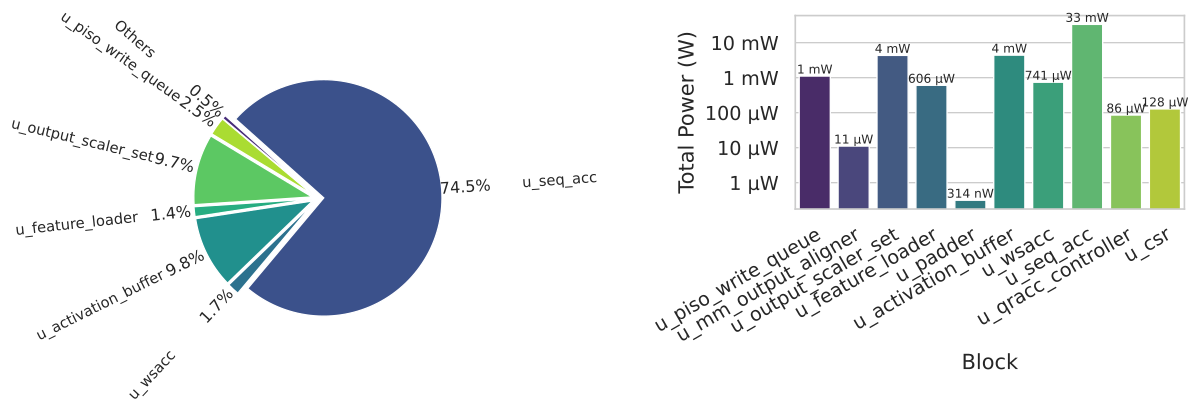
\includegraphics[width=\textwidth]{images/qracc/power_results.png}
    \caption{QRAcc Power Distribution}
    \label{fig:qracc_power_distribution}
\end{figure}

Figure \ref{fig:qracc_power_distribution} shows QRAcc's power distribution. The ACTMEM, being an SRAM bank, consumes a significant amount of power at $4uW$ as expected from memory. Next, the output scalers come at second with $3.6uW$. The output scalers consume power intensely due to having 8-bit multipliers each, and also being the critical path as they're purely combinational required large sizing and thus higher leakage and dynamic energy.  The SeqAcc core consumes the third most power at $1.1uW$ for its digital portion (but in fact, would consume the most power overall due to its analog portions). The main digital contributions to SeqAcc powercomes from the shift-multiplies and having the largest number of internal registers. 

\begin{figure}[htbp]
    \centering
    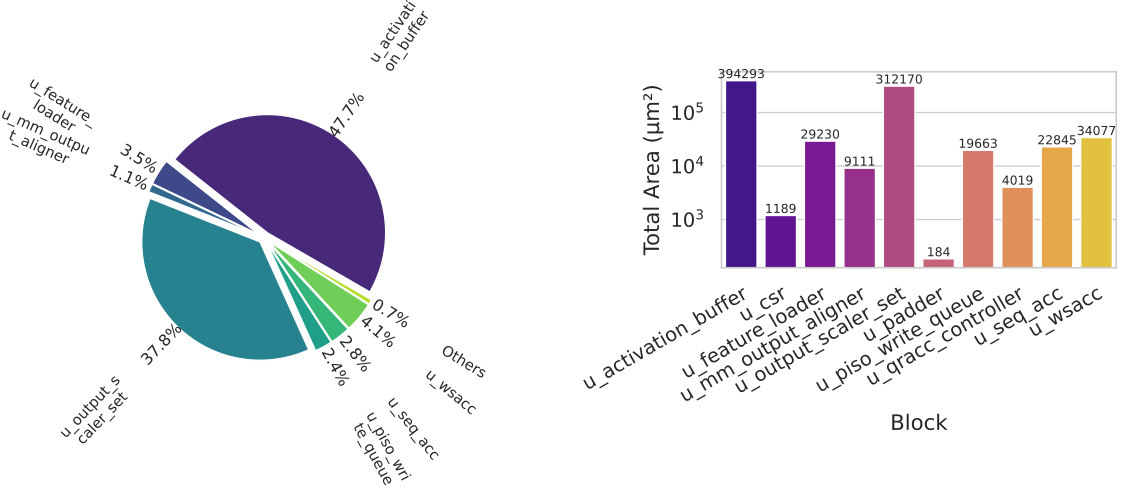
\includegraphics[width=\textwidth]{images/qracc/area_results.png}
    \caption{QRAcc Area Distribution}
    \label{fig:qracc_area_distribution}
\end{figure}

Figure \ref{fig:qracc_area_distribution} shows QRAcc's area distribution. The ACTMEM occupies the most area at $0.39mm^2$ which is due to it being made of 32 banks of $12.23um^2$ 8kB SRAMs. The output scalers come a close second at $0.3mm^2$ due to their utilization of 8b multipliers, barrel shifters, and large number of internal registers (256x32b bias registers, 256x16b scale and shift registers, 256x8b output offset registers). The WSAcc, FL, Write Queues, and SeqAcc all consume in the order of $10-100kum^2$ since they all utilize internal registers- 256x8b for the FL, 256x16b accumulators for the SeqAcc, 32x8b weight registers for WSAcc, and 8x(256+13)b shift registers for the write queues. Barrel shifters and address multiplexing also contribute significant remaining area to the FL, output aligner.

\subsection{State-dependent Power Consumption}

In order to account for an entire power and energy model of QRAcc, we also 
We do this by fully characterizing the state-dependent power consumption results of QRAcc. Table \ref{tab:qracc_state_power} shows the state-dependent power consumption (per Block) of QRAcc. Figure \ref{fig:qracc_state_power} shows the same data in a bar chart. By far, the Compute Analog state consumes the most power at $21.9 \mu W$. Compute Analog consumes this much power mainly due to the full use of the 256 output scaler blocks which are expensive due to their 16x8b array multipliers and barrel shifters. The Compute Digital state comes at second with $10.6 \mu W$, which is expected since it also uses the output scalers and also the WSacc core which also contains 32 8b multipliers.

\begin{table}[]
\centering
\label{tab:qracc_state_power}
\caption{QRAcc State-dependent Power Consumption in W}
\resizebox{\columnwidth}{!}{%
\begin{tabular}{c|rrrrrrrrr|r}
\cline{2-10}
 &
  \multicolumn{9}{c|}{\textbf{State}} &
  \multicolumn{1}{l}{} \\ \hline
\multicolumn{1}{|c|}{\textbf{Module}} &
  \multicolumn{1}{c}{\textbf{\begin{tabular}[c]{@{}c@{}}Compute\\ Analog\end{tabular}}} &
  \multicolumn{1}{c}{\textbf{\begin{tabular}[c]{@{}c@{}}Compute\\ Digital\end{tabular}}} &
  \multicolumn{1}{c}{\textbf{Idle}} &
  \multicolumn{1}{c}{\textbf{\begin{tabular}[c]{@{}c@{}}Load\\ Acts\end{tabular}}} &
  \multicolumn{1}{c}{\textbf{\begin{tabular}[c]{@{}c@{}}Load\\ Bias\end{tabular}}} &
  \multicolumn{1}{c}{\textbf{\begin{tabular}[c]{@{}c@{}}Load \\ Scalers\end{tabular}}} &
  \multicolumn{1}{c}{\textbf{\begin{tabular}[c]{@{}c@{}}Load \\ Weights\end{tabular}}} &
  \multicolumn{1}{c}{\textbf{\begin{tabular}[c]{@{}c@{}}Load \\ Weights \\ (WSAcc)\end{tabular}}} &
  \multicolumn{1}{c|}{\textbf{\begin{tabular}[c]{@{}c@{}}Read \\ Acts\end{tabular}}} &
  \multicolumn{1}{c|}{\textbf{\begin{tabular}[c]{@{}c@{}}Average\\ Power\end{tabular}}} \\ \hline
\multicolumn{1}{|c|}{\begin{tabular}[c]{@{}c@{}}Activation\\ Memory\end{tabular}} &
  \cellcolor[HTML]{FFE59A}4.56E-06 &
  \cellcolor[HTML]{FFE59B}4.44E-06 &
  \cellcolor[HTML]{FFE59D}4.10E-06 &
  \cellcolor[HTML]{FFE59B}4.48E-06 &
  \cellcolor[HTML]{FFE59C}4.31E-06 &
  \cellcolor[HTML]{FFE59C}4.31E-06 &
  \cellcolor[HTML]{FFE59C}4.32E-06 &
  \cellcolor[HTML]{FFE59C}4.29E-06 &
  \cellcolor[HTML]{FFE59B}4.40E-06 &
  \multicolumn{1}{r|}{\cellcolor[HTML]{FFD666}4.36E-06} \\ \cline{1-1}
\multicolumn{1}{|c|}{\begin{tabular}[c]{@{}c@{}}Feature\\ Loader\end{tabular}} &
  \cellcolor[HTML]{FFEBB1}7.61E-07 &
  \cellcolor[HTML]{FFEBB2}6.50E-07 &
  \cellcolor[HTML]{FFF0C4}3.15E-07 &
  \cellcolor[HTML]{FFEFC3}3.21E-07 &
  \cellcolor[HTML]{FFEFC3}3.21E-07 &
  \cellcolor[HTML]{FFEFC3}3.21E-07 &
  \cellcolor[HTML]{FFEFC3}3.21E-07 &
  \cellcolor[HTML]{FFF0C3}3.20E-07 &
  \cellcolor[HTML]{FFEBB3}4.17E-07 &
  \multicolumn{1}{r|}{\cellcolor[HTML]{FFEDB9}4.16E-07} \\ \cline{1-1}
\multicolumn{1}{|c|}{\begin{tabular}[c]{@{}c@{}}Output\\ Aligner\end{tabular}} &
  \cellcolor[HTML]{FFF6DA}1.99E-07 &
  \cellcolor[HTML]{FFFDF5}5.63E-08 &
  \cellcolor[HTML]{FFFBF0}8.32E-08 &
  \cellcolor[HTML]{FFFFFD}1.37E-08 &
  \cellcolor[HTML]{FFFFFD}1.37E-08 &
  \cellcolor[HTML]{FFFFFC}1.65E-08 &
  \cellcolor[HTML]{FFFFFD}1.13E-08 &
  \cellcolor[HTML]{FFFFFD}1.13E-08 &
  \cellcolor[HTML]{FFFFFD}1.37E-08 &
  \multicolumn{1}{r|}{\cellcolor[HTML]{FFFFFF}4.65E-08} \\ \cline{1-1}
\multicolumn{1}{|c|}{\begin{tabular}[c]{@{}c@{}}Output \\ Scaler\end{tabular}} &
  \cellcolor[HTML]{FFD666}1.31E-05 &
  \cellcolor[HTML]{FFE8A5}2.73E-06 &
  \cellcolor[HTML]{FFE8A7}2.41E-06 &
  \cellcolor[HTML]{FFE8A7}2.39E-06 &
  \cellcolor[HTML]{FFE8A8}2.36E-06 &
  \cellcolor[HTML]{FFE8A8}2.37E-06 &
  \cellcolor[HTML]{FFE8A8}2.31E-06 &
  \cellcolor[HTML]{FFE8A8}2.34E-06 &
  \cellcolor[HTML]{FFE8A8}2.35E-06 &
  \multicolumn{1}{r|}{\cellcolor[HTML]{FFDB75}3.60E-06} \\ \cline{1-1}
\multicolumn{1}{|c|}{\begin{tabular}[c]{@{}c@{}}Padding\\ Module\end{tabular}} &
  \cellcolor[HTML]{FFF5D8}2.11E-07 &
  \cellcolor[HTML]{FFF9E6}1.36E-07 &
  \cellcolor[HTML]{FFFFFF}3.26E-10 &
  \cellcolor[HTML]{FFFFFF}5.01E-10 &
  \cellcolor[HTML]{FFFFFF}3.46E-10 &
  \cellcolor[HTML]{FFFFFF}3.46E-10 &
  \cellcolor[HTML]{FFFFFF}3.46E-10 &
  \cellcolor[HTML]{FFFFFF}3.46E-10 &
  \cellcolor[HTML]{FFFBEF}8.74E-08 &
  \multicolumn{1}{r|}{\cellcolor[HTML]{FFFFFF}4.85E-08} \\ \cline{1-1}
\multicolumn{1}{|c|}{\begin{tabular}[c]{@{}c@{}}Write\\ Queue\end{tabular}} &
  \cellcolor[HTML]{FFEBB1}7.76E-07 &
  \cellcolor[HTML]{FFEBB2}6.34E-07 &
  \cellcolor[HTML]{FFEBB3}5.60E-07 &
  \cellcolor[HTML]{FFEBB2}5.69E-07 &
  \cellcolor[HTML]{FFEBB2}5.68E-07 &
  \cellcolor[HTML]{FFEBB2}5.68E-07 &
  \cellcolor[HTML]{FFEBB2}5.68E-07 &
  \cellcolor[HTML]{FFEBB3}5.64E-07 &
  \cellcolor[HTML]{FFEBB2}5.66E-07 &
  \multicolumn{1}{r|}{\cellcolor[HTML]{FFEBB1}5.97E-07} \\ \cline{1-1}
\multicolumn{1}{|c|}{Controller} &
  \cellcolor[HTML]{FFFDF5}5.54E-08 &
  \cellcolor[HTML]{FFFDF6}5.26E-08 &
  \cellcolor[HTML]{FFFDF6}5.07E-08 &
  \cellcolor[HTML]{FFFDF7}4.65E-08 &
  \cellcolor[HTML]{FFFDF7}4.57E-08 &
  \cellcolor[HTML]{FFFDF7}4.57E-08 &
  \cellcolor[HTML]{FFFDF7}4.62E-08 &
  \cellcolor[HTML]{FFFDF7}4.55E-08 &
  \cellcolor[HTML]{FFFDF7}4.59E-08 &
  \multicolumn{1}{r|}{\cellcolor[HTML]{FFFFFF}4.82E-08} \\ \cline{1-1}
\multicolumn{1}{|c|}{\begin{tabular}[c]{@{}c@{}}SeqAcc\\ (Digital)\end{tabular}} &
  \cellcolor[HTML]{FFE9AB}1.83E-06 &
  \cellcolor[HTML]{FFEAB0}1.02E-06 &
  \cellcolor[HTML]{FFEBB0}1.00E-06 &
  \cellcolor[HTML]{FFEAB0}1.01E-06 &
  \cellcolor[HTML]{FFEAB0}1.01E-06 &
  \cellcolor[HTML]{FFEAB0}1.01E-06 &
  \cellcolor[HTML]{FFEAB0}1.02E-06 &
  \cellcolor[HTML]{FFEAB0}1.01E-06 &
  \cellcolor[HTML]{FFEAB0}1.01E-06 &
  \multicolumn{1}{r|}{\cellcolor[HTML]{FFE8A7}1.10E-06} \\ \cline{1-1}
\multicolumn{1}{|c|}{WSAcc} &
  \cellcolor[HTML]{FFEBB3}4.01E-07 &
  \cellcolor[HTML]{FFEBB0}9.00E-07 &
  \cellcolor[HTML]{FFEDB9}3.73E-07 &
  \cellcolor[HTML]{FFECB5}3.91E-07 &
  \cellcolor[HTML]{FFECB6}3.89E-07 &
  \cellcolor[HTML]{FFECB6}3.89E-07 &
  \cellcolor[HTML]{FFECB6}3.89E-07 &
  \cellcolor[HTML]{FFEBB3}4.01E-07 &
  \cellcolor[HTML]{FFECB4}3.98E-07 &
  \multicolumn{1}{r|}{\cellcolor[HTML]{FFEBB3}4.48E-07} \\ \hline
\multicolumn{1}{|c|}{\begin{tabular}[c]{@{}c@{}}Total\\ Power\end{tabular}} &
  \cellcolor[HTML]{FFD666}2.19E-05 &
  \cellcolor[HTML]{FFE9AA}1.06E-05 &
  \cellcolor[HTML]{FFFFFF}8.89E-06 &
  \cellcolor[HTML]{FFEBB2}9.22E-06 &
  \cellcolor[HTML]{FFEDBB}9.02E-06 &
  \cellcolor[HTML]{FFEBB3}9.03E-06 &
  \cellcolor[HTML]{FFF2CC}8.99E-06 &
  \cellcolor[HTML]{FFF2CE}8.98E-06 &
  \cellcolor[HTML]{FFEBB2}9.29E-06 &
  \multicolumn{1}{r|}{1.07E-05} \\ \hline
\end{tabular}%
}
\end{table}

\begin{figure}[htbp]
    \centering
    \includegraphics[width=\textwidth]{images/qracc/state_power_consumption.png}
    \caption{QRAcc Per-state Power Consumption}
    \label{fig:qracc_state_power}
\end{figure}

\section{Conclusion}

In this chapter, we presented QRAcc, a charge-redistribution SRAM-based AIMC accelerator for DNNs. QRAcc is a fully integrated AIMC accelerator that can perform both analog and digital computations. It uses SeqAcc as its main analog core and WSAcc as its digital core. QRAcc achieves a peak energy efficiency of 516.1 TOPS/W at 409.6 GOPS, which is comparable to state-of-the-art.

In the next chapter, we will present the results of optimizing DNN mappings on QRAcc with MARP.
\chapter{MARP Results with QRAcc}

In this chapter, we present the benefits of using MARP on QRAcc, our hybrid AIMC accelerator architecture. MARP can achieve a 26.19\% reduction in energy consumption and a 19.65\% reduction in latency on MobileNetV2 inference in QRAcc.  

\label{chap:marp_qracc}

\section{Extracting Statistics from QRAcc}

We compile and perform inference on the MLPerfTiny models using MARP, while at the same time tracking statistics in a global data structure. QRAcc's individual RTL blocks fill up the statistics data structure during behavioral simulation. Every new layer, the statistics data structure is exported into a CSV row and then cleared for the next layer. The statistics data structure contains the following fields:

\begin{enumerate}
    \item \texttt{statActmem...}: Counts read and write operations to the Activation Memory, distinguishing between internal and external port access.
    \item \texttt{statFL...}: Counts read and write operations to the Free List memory.
    \item \texttt{statSeqAcc...}: Tracks operations related to the Sequential Accumulator, including weight writes, total operations, and the number of Multiply-Accumulate (MAC) operations.
    \item \texttt{statWQ...}: Counts read and write operations to the Weight Queue.
    \item \texttt{cyclesIdle}: Number of cycles the accelerator was idle.
    \item \texttt{cyclesLoad...}: Cycles spent on loading data, such as activations, scalers, biases, and weights for both analog and digital units.
    \item \texttt{cyclesCompute...}: Cycles spent on computation, separated into analog and digital processing phases.
    \item \texttt{cyclesReadActivation}: Cycles consumed while reading out the resulting activations from the memory.
\end{enumerate}

Given the characterizations on QRAcc in Chapter \ref{chap:qracc} and the tracked statistics, we calculate the energy consumption of QRAcc. For most of the state-dependent energy components, 

\begin{equation}
    E_{state} = P_{qracc,state}\cdot N_{cycles,state}\cdot T_{clk}
\end{equation}

where $T_{clk}$ is 50MHz. For the "Load Weights" state in particular, we use the following equation:
\begin{equation}
    E_{load\_weights} = N_{cycles,load\_weights}\cdot T_{clk}(32\cdot P_{seqacc,write,bit}\cdot P_{qracc,load\_weights})
\end{equation}

where $P_{seqacc,write,per-bit}$ is power consumed by writing a single bit to SeqAcc as measured in Chapter \ref{chap:qracc}. SeqAcc writes 32 bits per cycle, so we multiply by 32. $P_{qracc,load\_weights}$ is the power consumed by the QRAcc architecture when loading weights, which was measured in Chapter \ref{chap:qracc}.

Lastly, for the "Compute Analog" state, we use the following equation:
\begin{equation}
    E_{analog} = N_{cycles,analog}\cdot T_{clk}(K\cdot P_{seqacc,mac,column}\cdot P_{qracc,analog})
\end{equation}

where $K$ is the number of output channels of the layer being computed, and the rest are values we measured in Chapter \ref{chap:qracc}. We scale the power by $K$ because SeqAcc only activates $K$ columns when only $K$ output channels are computed. 

\section{Latency Results}

\begin{figure}[htbp]
    \centering
    \includegraphics[width=\textwidth]{images/marp_qracc/timeline.png}
    \caption{Line plot of the total inference time vs node being processed in QRAcc for inference in each of the 4 MLPerfTiny models. At the end of the lines, we annotate the reduction in inference time vs the naive single-mapping packer.}
    \label{fig:timeline}
\end{figure}

\begin{figure}[htbp]
    \centering
    \includegraphics[width=\textwidth]{images/marp_qracc/time_bars.png}
    \caption{Stacked bar chart of the time spent in each state of QRAcc for inference in each of the 4 MLPerfTiny models}
    \label{fig:time_bars}
\end{figure}

Figure \ref{fig:timeline} shows the total inference time vs node being processed in QRAcc for inference in each of the 4 MLPerfTiny models. The lines show the total inference time for each node, and at the end of the lines, we annotate the reduction in inference time vs the naive single-mapping packer. We see that of the packers, the naive packer tends to take the longest inference time, then the balanced packer, then the write-optimized packer.

The main cause of the reduction in inference time can be seen by taking a look at Figure \ref{fig:time_bars}, which shows a stacked bar chart of the time spent in each state of QRAcc for inference in each of the 4 MLPerfTiny models. For all of the models' naive single-mapping, the "Load Weights" state takes the longest due to the large number of writes to the SeqAcc memory array. As the packer used optimizes for less writes, the "Load Weights" state takes less time and this is reflected in the total inference time. 

For the FC-AE and DS-CNN models, they tend to have much a higher number of smaller matrices than the other models. Hence, the latency reductions on these models are massive at -44.4\% and -57.85\%. However, MARP on these models retains the same number of bins for all 4 packers, so the reduction in inference time is the same for all the packings. Interestingly, the time spent loading weights dominates in FC-AE inference. We attribute this to the fact that FC-AE is a model made up of mostly fully-connected layers, which turn into simple matrix multiplications. This is equivalent to a pointwise convolution with a 1x1 image with 640 input channels and 640 output channels. Since there is only one pixel to process, the computation time is extremely short compared to the time spent loading weights.

For the MobileNetV2 model, we see more distinction in the different packers. On MobileNetV2, despite the dense packer being able to reduce the bins from 91 to 34, the dense packing has such a random access pattern that the number of writes is essentially the same as the naive single-mapping packer leading to a very low reduction in inference time of -2.12\%. On the other hand the balanced and write-optimized packers are able to reduce the number of writes instead of just the number of bins, leading to a reduction in inference time of -10.62\% and -19.65\% respectively.

For the ResNet model, we see that even the dense packer is able to reduce the inference time by as much as -27.66\% which we attribute to the sheer amount of utilization gained. From 15 bins, all of the packers of the ResNet model are able to reduce the number of bins to 2, which leads to a significant reduction in the number of writes to the SeqAcc memory array. The balanced packer and write-optimized packer are further able to make sure to use the same bin for consecutive layers, which leads to a further reduction in inference time of -35.56\% and -47.41\% respectively.

\section{Energy Results}

\begin{figure}[htbp]
    \centering
    \includegraphics[width=\textwidth]{images/marp_qracc/energy_bars.png}
    \caption{Stacked bar chart of the energy used for inference in each of the 4 MLPerfTiny models}
    \label{fig:energy_bars}
\end{figure}

\begin{figure}[htbp]
    \centering
    \includegraphics[width=\textwidth]{images/marp_qracc/tops_bars.png}
    \caption{Stacked bar chart of the energy efficiency (TOPS/W) of QRAcc for inference in each of the 4 MLPerfTiny models}
    \label{fig:tops_bars}
\end{figure}

Figure \ref{fig:energy_bars} shows a stacked bar chart of the energy used for inference in each of the 4 MLPerfTiny models. We see that for all the models, the naive single-mapping packer uses the most energy per inference, followed by the dense packer, then the balanced packer, and finally the write-optimized packer. The main reason for the energy savings is the same as the latency savings: the reduction in the number of writes to the SeqAcc memory array. By skipping the load weights state whenever the previously loaded bin into QRAcc is the bin of the current layer, we can save on all of the write energy.

The FC-AE and DS-CNN models show the most energy savings as with the latency results. MARP reduced the FC-AE and DS-CNN energy consumptions by -55.79\% and -59.52\% respectively. This is a higher gain than the latency results because the energy consumed by the "Load Weights" state is higher than the latency added by it. Again, for the different packers, MARP obtains no significant difference in energy savings owing to the fact that packing allows the use of very few bins (1 for FC-AE and 2 for DS-CNN).

For the MobileNetV2 model, we see that the dense packer is able to reduce the energy consumption by only -2.83\% compared to the naive single-mapping packer. However, the balanced and write-optimized packers are able to reduce the energy consumption by -14.16\% and -26.19\% respectively. There are lower reductions in energy consumption for MobileNetV2 due to its massive layer matrix sizes, as there are still many writes to the SeqAcc memory array even with packings. Not only that, but a significant number of the layers in MobileNetV2 are depthwise convolutions, which are mapped to the digital core of QRAcc. This portion of the energy consumption is not reduced by MARP, as MARP only optimizes the AIMC core of QRAcc.

Lastly, for the ResNet model, we see that the dense packer is able to reduce the energy consumption by -29.65\% compared to the naive single-mapping packer. The balanced packer and write-optimized packer are able to reduce the energy consumption by -38.12\% and -50.83\% respectively. The ResNet model has a very high number of layers and unlike MobileNetV2, it does not have depthwise convolutions. This means that the majority of the layers are mapped to the SeqAcc memory array, which allows MARP to reduce the number of writes to the SeqAcc memory array significantly. However, we still see the benefits of the write-optimized packer due to the number of bins (16) needed for the ResNet model. Having a higher number of bins means that there is a higher chance that the next layer will not be in the same bin as the previous layer, which the write-optimized packer is able to optimize for.

Figure \ref{fig:tops_bars} shows a stacked bar chart of the energy efficiency (TOPS/W) of QRAcc for inference in each of the 4 MLPerfTiny models. Note that this energy efficiency is expected to be lower than that reported in Chapter \ref{chap:qracc} because the energy efficiency reported in Chapter \ref{chap:qracc} is the peak energy efficiency of QRAcc, while this is the energy efficiency of practical inference, accounting for the energy consumed while moving data into QRAcc as well.

We see MARP allows the energy efficiency for all the models go to at least around 5 TOPS/W or above, which is relatively efficient even including the energy consumption of data movement. While these energy efficiency values are lower than what would usually be expected, it is high if you consider that these are system-level measurements. In existing literature, most of the high energy efficiency values are reported on the bank level (for AIMCs) and L2-array level (for digital accelerators). 

These levels of energy efficiency can enable the use of QRAcc in edge AI applications, which was the main goal of this work. 

\section{Influence of Layer Type}

We further analyze the influence of layer type such as depthwise, input feature map sizes, kernel sizes, and node order on the performance. Figure \ref{fig:duration_tops_scatter} shows a scatter plot of the latency vs energy of different layers in the MLPerfTiny models. The sizes of the markers in the scatter plot represent the size of the input feature map of the layer, while the colors represent the size of the kernel. Cross-marks are depthwise convolutions, while circles are regular convolutions and matrix multiplications.

We see that layers with larger input feature maps tend to take longer (but not always) to process, which is expected as larger input feature maps require more computations. However, we also see that they can also obtain very high energy efficiencies when MARP packs then with high emphasis on the write optimization. 

We also see that depthwise convolutions tend to take much faster to process than regular convolutions and matrix multiplications. This is as expected, as they are composed of much fewer MACs and operations than regular convolutions and matrix multiplications. However, we can also see that the energy efficiencies of calculating them are around the same as that of the regular convolutions and matrix multiplications. With the naive and dense packers, the energy efficiency of depthwise convolutions is sometimes higher than that of regular convolutions and matrix multiplications. However, as we optimize for writing in the AIMC array less, the energy efficiency of most of the regular convolutions are now competitive with the depthwise convolutions.

\begin{figure}[htbp]
    \centering
    \includegraphics[width=\textwidth]{images/marp_qracc/duration_tops_scatter.png}
    \caption{Scatter plot of the energy vs latency of different layers in the MLPerfTiny models}
    \label{fig:duration_tops_scatter}
\end{figure}

% \section{Hardware Overhead}

% MARP required special hardware (see QRAcc motivations in Chapter \ref{chap:qracc}) to provide the alignment of row inputs and column outputs to the mapped matrix in the AIMC memory array. In terms of the required designs, the feature loader's fundamental design as a register file allows alignment of row inputs to the mapped matrix in the AIMC memory array. Then, an aligner fixes the column output alignment at the end, which is the only datapath overhead of MARP. 

% The feature loader's design, while allowing the row offsets required by MARP, is not easily factored into an "offset-allowing" portion and one that is not. This is because the way we designed the feature loader needs to be able feature loader to be able to load the features in a way that allows for any row offset. Hence, the feature loader is not a MARP-specific design, but rather a design that works well with MARP.

% The output aligner is the only true overhead of MARP. However, we showed in Figure \ref{fig:qracc_area_distribution} that the output aligner only accounts for 1.1\% of the total area of QRAcc. This is a very small overhead compared to the overall area of QRAcc, which is dominated by the SeqAcc memory array and the WSAcc digital core. Furthermore, this area contribution does not even account for the area of the SeqAcc memory array, which is the main component of QRAcc. 

% Hence, the hardware overhead of MARP is minimal and does not significantly impact the overall performance of the QRAcc architecture.

\section{Conclusion}

In this chapter, we presented the results of MARP on QRAcc, our hybrid AIMC accelerator architecture. MARP achieves significant improvements in energy efficiency and inference latency across various MLPerfTiny models, with an average energy consumption reduction of 26.19\% and latency reduction of 19.65\% for MobileNetV2 inference. The statistics extraction method from QRAcc was detailed, alongside the energy and latency results that showcase the advantages of using MARP. The findings indicate that MARP's optimization strategies are effective in enhancing the performance of hybrid AIMC architectures like QRAcc, making them more suitable for edge AI applications.

We'd like to note that we demonstrated MARP with QRAcc in this chapter. However, it can be applied to many other AIMC accelerators. For AIMC accelerators that use multibit non-volatile memories that take a lot of write energy and latency, we believe that MARP will be even better for them. Multibit AIMC memories like PCM and RRAM take a lot of write energy and latency (due to the write-verify method), which MARP can significantly reduce. Furthermore, QRAcc only supports 1b weights at the moment. If QRAcc were to support multibit weights, we would be able to further show reduction as there will be more weights to write.
\section{Conclusion}

Existing DNN mappers for AIMC accelerators are limited to single-mapping schemes, which significantly wastes the available space in the AIMC memory array. In this work, we introduced MARP, a DNN mapper that can optimize the mapping of multiple layers in AIMC accelerators with interlayer weight reuse. MARP uses rectangular bin packing algorithms to pack multiple DNN layers into a single matrix written into the AIMC, optimizing the utilization of the AIMC architecture.

MARP was able to increase the utilizations of the AIMC memory arrays of the MLPerfTiny models. Compared to the single-mapping schemes of existing DNN mappers, MARP's dense packing was able to increase the AIMC memory utilization by 25.07\% for DS-CNN, 51.84\% for FC-AE, 45.71\% for MobileNetV2, and 64.7\% for ResNet. 
We also discovered that, by utilizing the online variants of the rectangular bin packing algorithms, MARP can also reduce the number of AIMC memory writes needed in inference. MARP reduced the number of AIMC memory writes in MobileNetV2 by 41.3\%, in DS-CNN by 71.43\%, in FC-AE by 60.0\%, and in ResNet by 81.25\%.

MARP-Dense's ability to reduce the number of bins allows AIMC accelerators with a large number of cores to fully map models like MobileNetV2. For example, NeuRRAM's 48 cores can already fully map the MARP-Dense packing of MobileNetV2 at 34 bins. 

To demonstrate the effectiveness of MARP, we also introduced QRAcc, a charge-redistribution SRAM-based AIMC accelerator for DNNs. QRAcc is a fully integrated AIMC accelerator that can perform both analog and digital computations. It uses SeqAcc as its main analog core and WSAcc as its digital core. QRAcc achieves a peak energy efficiency of 509.3 peak TOPS/W at 6.55 TOPS with its AIMC core, which is comparable to state-of-the-art. With its digital core WSAcc, QRAcc achieves a peak energy efficiency of 81.356 peak TOPS/W at 5.76 GOPS, which is also comparable to state-of-the-art digital accelerators.

We evaluated the integration of MARP with the QRAcc AIMC accelerator, demonstrating the practical benefits of MARP’s mapping strategies on real hardware. By leveraging MARP’s optimized layer packing and interlayer weight reuse, QRAcc achieved significant improvements in memory utilization and computational efficiency across a range of MLPerfTiny models. The results show that MARP-enabled QRAcc not only reduces the number of memory writes and increases array utilization, but also sustains significant gains in energy efficiency (up to 1723.2\% on the MLPerfTiny models), energy consumption (up to 59.52\% lower energy consumption) and throughput (up to 57.87\% reduction), validating the effectiveness of MARP’s approach in a state-of-the-art AIMC system.

\section{Future Work}

Due to the success of MARP in optimizing AIMC mappings, we believe that the next step in the evolution of existing DNN mappers is to implement schemes like MARP's rectangular packing that can account for the spatial reuse of memory cells in AIMC accelerators. Paired with their existing memory access optimizations, we believe that SOTA DNN mappers like ZigZag/Stream, TimeLoop/CIMLoop, and LionHeart can achieve even higher AIMC memory utilization and energy efficiencies. 

For QRAcc, we'd like to next analyze its compute SNR performance as co-designed with the ONNX splittings that are necessary to fit the layers in. QRAcc also only supports 1b weights for the purposes of this work. We would like to extend QRAcc to support multibit weights.

\backmatter
\printbibliography
% bibliography, glossary and index would go here.

\chapter*{Appendix}

\section{SeqAcc Operation}
\label{section:appendixseqacc}

\subsection{Charge Redistribution}

take from y2q1 

\subsection{Write and Read}

could be taken from the early Y2Q2 report

\subsection{ADC Design}

take from Y2Q3 report

\subsection{QRAcc Bitcell Design}

can take from the early Y2Q1 report

Lorem Ipsum dolor sit amet, consectetur adipiscing elit. Sed do eiusmod tempor incididunt ut labore et dolore magna aliqua. Ut enim ad minim veniam, quis nostrud exercitation ullamco laboris nisi ut aliquip ex ea commodo consequat. Duis aute irure dolor in reprehenderit in voluptate velit esse cillum dolore eu fugiat nulla pariatur. Excepteur sint occaecat cupidatat non proident, sunt in culpa qui officia deserunt mollit anim id est laborum.

\section{QLinear Operations}
\label{section:appendixqlinearops}
Lorem Ipsum dolor sit amet, consectetur adipiscing elit. Sed do eiusmod tempor incididunt ut labore et dolore magna aliqua. Ut enim ad minim veniam, quis nostrud exercitation ullamco laboris nisi ut aliquip ex ea commodo consequat. Duis aute irure dolor in reprehenderit in voluptate velit esse cillum dolore eu fugiat nulla pariatur. Excepteur sint occaecat cupidatat non proident, sunt in culpa qui officia deserunt mollit anim id est laborum.

\section{QRAcc CSRs and Configuration Registers}
\label{section:appendixqracc_csrs}
\begin{longtable}{@{}llll@{}}
\caption{CSR 0: Main Control Register Bit Fields} \\
\toprule
Bits & Field Name & R/W & Description \\ \midrule
\endfirsthead
\multicolumn{4}{c}%
{{\bfseries \tablename\ \thetable{} -- continued from previous page}} \\
\toprule
Bits & Field Name & R/W & Description \\ \midrule
\endhead
\bottomrule
\endfoot
\endlastfoot
2:0 & \texttt{csr\_main\_trigger} & W & Main trigger for the controller. See Table \ref{tab:triggers}. \\
3 & \texttt{csr\_main\_clear} & W & Clears the controller state. \\
4 & \texttt{csr\_main\_busy} & R & Indicates if the controller is not in the idle state. \\
5 & \texttt{inst\_write\_mode} & W & Set to 1 if writing instructions for a microcode loop. \\
11:8 & \texttt{internal\_state} & R & The internal state of the controller FSM for debugging. \\
12 & \texttt{preserve\_ifmap} & W & If set, the input feature map is preserved after computation. \\
\end{longtable}

\begin{longtable}{@{}llll@{}}
\caption{CSR 1: Layer Configuration Register Bit Fields} \\
\toprule
Bits & Field Name & R/W & Description \\ \midrule
\endfirsthead
\multicolumn{4}{c}%
{{\bfseries \tablename\ \thetable{} -- continued from previous page}} \\
\toprule
Bits & Field Name & R/W & Description \\ \midrule
\endhead
\bottomrule
\endfoot
\endlastfoot
0 & \texttt{binary\_cfg} & W & 1 for binary mode, 0 for bipolar mode. \\
1 & \texttt{unsigned\_acts} & W & 1 for unsigned activations, 0 for signed. \\
7:4 & \texttt{adc\_ref\_range\_shifts} & W & ADC reference range shifts. \\
11:8 & \texttt{filter\_size\_y} & W & Filter dimension in the Y direction. \\
15:12 & \texttt{filter\_size\_x} & W & Filter dimension in the X direction. \\
19:16 & \texttt{stride\_y} & W & Stride in the Y direction. \\
23:20 & \texttt{stride\_x} & W & Stride in the X direction. \\
27:24 & \texttt{n\_input\_bits\_cfg} & W & Number of bits for input data. \\
31:28 & \texttt{n\_output\_bits\_cfg} & W & Number of bits for output data. \\
\end{longtable}

\begin{longtable}{@{}lllll@{}}
\caption{CSR 2 \& 3: Feature Map Dimension Bit Fields} \\
\toprule
Register & Bits & Field Name & R/W & Description \\ \midrule
\endfirsthead
\multicolumn{5}{c}%
{{\bfseries \tablename\ \thetable{} -- continued from previous page}} \\
\toprule
Register & Bits & Field Name & R/W & Description \\ \midrule
\endhead
\bottomrule
\endfoot
\endlastfoot
CSR 2 & 15:0 & \texttt{input\_fmap\_dimx} & W & Input fmap dimension X. \\
CSR 2 & 31:16 & \texttt{input\_fmap\_dimy} & W & Input fmap dimension Y. \\
CSR 3 & 15:0 & \texttt{output\_fmap\_dimx} & W & Output fmap dimension X. \\
CSR 3 & 31:16 & \texttt{output\_fmap\_dimy} & W & Output fmap dimension Y. \\
\end{longtable}

\begin{longtable}{@{}llll@{}}
\caption{CSR 4: Channel Configuration Bit Fields} \\
\toprule
Bits & Field Name & R/W & Description \\ \midrule
\endfirsthead
\multicolumn{4}{c}%
{{\bfseries \tablename\ \thetable{} -- continued from previous page}} \\
\toprule
Bits & Field Name & R/W & Description \\ \midrule
\endhead
\bottomrule
\endfoot
\endlastfoot
15:0 & \texttt{num\_input\_channels} & W & Number of input channels. \\
31:16 & \texttt{num\_output\_channels} & W & Number of output channels. \\
\end{longtable}

\begin{longtable}{@{}llll@{}}
\caption{CSR 5: Mapped Matrix Offset Bit Fields} \\
\toprule
Bits & Field Name & R/W & Description \\ \midrule
\endfirsthead
\multicolumn{4}{c}%
{{\bfseries \tablename\ \thetable{} -- continued from previous page}} \\
\toprule
Bits & Field Name & R/W & Description \\ \midrule
\endhead
\bottomrule
\endfoot
\endlastfoot
15:0 & \texttt{mapped\_matrix\_offset\_x} & W & Mapped matrix offset in X. \\
31:16 & \texttt{mapped\_matrix\_offset\_y} & W & Mapped matrix offset in Y. \\
\end{longtable}

\begin{longtable}{@{}llll@{}}
\caption{CSR 6: Padding Information Bit Fields} \\
\toprule
Bits & Field Name & R/W & Description \\ \midrule
\endfirsthead
\multicolumn{4}{c}%
{{\bfseries \tablename\ \thetable{} -- continued from previous page}} \\
\toprule
Bits & Field Name & R/W & Description \\ \midrule
\endhead
\bottomrule
\endfoot
\endlastfoot
3:0 & \texttt{padding} & W & Set to 1 to enable zero-padding. \\
11:4 & \texttt{padding\_value} & W & Value to use for padding. \\
\end{longtable}



\section{On the possibility of masking writes instead of reducing bins}
\label{section:appendixmasking_writes}

In cases of regular non-bitmasking enabled SRAM, this idea is impossible. However, if the SRAM is bitmasking enabled, it is possible to mask writes to the SRAM. Then, it is possible to only write the useful portions of the matrices onto the SRAM. Combined with QRAcc's column and row masking, this can work as an alternative to MARP while still making use of powerful system-level optimizing single-mapping DNN compilers like CIMLoop, LionHeart, and ZigZag. 

We need QRAcc's row and column masking because with a bitmasking scheme, large matrices left over in the AIMC memory array will not be overwritten by zeros. If the inputs and outputs of those portions are not masked away, (1) unnecessary computational power will be utilized (if the inputs are not maskeed) and (2) the outputs will be incorrect (if the outputs are not masked).

I believe this is actually a pretty good idea for future work. It would allow the use of existing DNN compilers that do not support multi-mapping, while still optimizing for the fewest possible writes.

On the other hand, MARP is also able to solve mappings for multicore AIMC accelerators for whom all the matrices are loaded in all at once. This is not possible with the masking scheme, as the masking scheme essentially evicts the matrices that are not needed for the current inference.

\section{Extra MARP experiments}
\label{section:appendixextra_marp_experiments}

\begin{figure}[htbp]
    \centering
    \includegraphics[width=\textwidth]{images/appendix/mlperftiny_utilization_vs_packer.png}
    \caption{Utilization achieved on the MLPerfTiny models for various variants of the MaxRects (MR) algorithm. Different rectpack variants achieve utilizations, but using rectangular packing always improves both compared to single-mapping.}
\end{figure}

\begin{figure}[htbp]
    \centering
    \includegraphics[width=\textwidth]{images/appendix/marp_multicore.png}
    \caption{Multicore experiments with MARP for MobileNetV2}
\end{figure}


\section{SNR Analysis of QRAcc}
\label{section:appendixsnr_analysis}

already in y2q3 report

\subsection{Per-layer SNR on MBV2}

raw data already there, analysis needed.

\end{document}